\documentclass[]{book}
\usepackage{lmodern}
\usepackage{amssymb,amsmath}
\usepackage{ifxetex,ifluatex}
\usepackage{fixltx2e} % provides \textsubscript
\ifnum 0\ifxetex 1\fi\ifluatex 1\fi=0 % if pdftex
  \usepackage[T1]{fontenc}
  \usepackage[utf8]{inputenc}
\else % if luatex or xelatex
  \ifxetex
    \usepackage{mathspec}
  \else
    \usepackage{fontspec}
  \fi
  \defaultfontfeatures{Ligatures=TeX,Scale=MatchLowercase}
\fi
% use upquote if available, for straight quotes in verbatim environments
\IfFileExists{upquote.sty}{\usepackage{upquote}}{}
% use microtype if available
\IfFileExists{microtype.sty}{%
\usepackage{microtype}
\UseMicrotypeSet[protrusion]{basicmath} % disable protrusion for tt fonts
}{}
\usepackage{hyperref}
\hypersetup{unicode=true,
            pdftitle={Math 115: Elementary Statistics},
            pdfauthor={Rong You},
            pdfborder={0 0 0},
            breaklinks=true}
\urlstyle{same}  % don't use monospace font for urls
\usepackage{natbib}
\bibliographystyle{apalike}
\usepackage{longtable,booktabs}
\usepackage{graphicx,grffile}
\makeatletter
\def\maxwidth{\ifdim\Gin@nat@width>\linewidth\linewidth\else\Gin@nat@width\fi}
\def\maxheight{\ifdim\Gin@nat@height>\textheight\textheight\else\Gin@nat@height\fi}
\makeatother
% Scale images if necessary, so that they will not overflow the page
% margins by default, and it is still possible to overwrite the defaults
% using explicit options in \includegraphics[width, height, ...]{}
\setkeys{Gin}{width=\maxwidth,height=\maxheight,keepaspectratio}
\IfFileExists{parskip.sty}{%
\usepackage{parskip}
}{% else
\setlength{\parindent}{0pt}
\setlength{\parskip}{6pt plus 2pt minus 1pt}
}
\setlength{\emergencystretch}{3em}  % prevent overfull lines
\providecommand{\tightlist}{%
  \setlength{\itemsep}{0pt}\setlength{\parskip}{0pt}}
\setcounter{secnumdepth}{5}
% Redefines (sub)paragraphs to behave more like sections
\ifx\paragraph\undefined\else
\let\oldparagraph\paragraph
\renewcommand{\paragraph}[1]{\oldparagraph{#1}\mbox{}}
\fi
\ifx\subparagraph\undefined\else
\let\oldsubparagraph\subparagraph
\renewcommand{\subparagraph}[1]{\oldsubparagraph{#1}\mbox{}}
\fi

%%% Use protect on footnotes to avoid problems with footnotes in titles
\let\rmarkdownfootnote\footnote%
\def\footnote{\protect\rmarkdownfootnote}

%%% Change title format to be more compact
\usepackage{titling}

% Create subtitle command for use in maketitle
\providecommand{\subtitle}[1]{
  \posttitle{
    \begin{center}\large#1\end{center}
    }
}

\setlength{\droptitle}{-2em}

  \title{Math 115: Elementary Statistics}
    \pretitle{\vspace{\droptitle}\centering\huge}
  \posttitle{\par}
    \author{Rong You}
    \preauthor{\centering\large\emph}
  \postauthor{\par}
      \predate{\centering\large\emph}
  \postdate{\par}
    \date{2019-08-12}

\usepackage{booktabs}

\begin{document}
\maketitle

{
\setcounter{tocdepth}{1}
\tableofcontents
}
\hypertarget{chapter-1}{%
\chapter{Chapter 1}\label{chapter-1}}

\hypertarget{welcome}{%
\section{Welcome}\label{welcome}}

\begin{itemize}
\tightlist
\item
  Always check Canvas for everything (homework assignments, announcements, grades, and etc.. )
\item
  Please send me emails directly using your avc email. Don't send me emails through the Canvas system because Canvas doesn't handle attachments well.
\item
  Syllabus
\item
  Questions?
\end{itemize}

\hypertarget{statistical-and-critical-thinking}{%
\section{Statistical and Critical Thinking}\label{statistical-and-critical-thinking}}

\begin{itemize}
\tightlist
\item
  \emph{Statistics}: The science of planning studies and experiments, obtaining data, and then organizing, summarizing, presenting, analyzing, interpreting, and drawing conclusions based on the data. \href{https://www.youtube.com/watch?v=nTBZuQR7dRc}{What does statistics do?}
\item
  \emph{Data}: Collections of observations, such as measurements, genders, or survey responses
\item
  \emph{Population}: The complete collection of \textbf{all} measurements or data that are being considered. Typically, a population is the complete collection of data that we would like to make inferences about.
\item
  \emph{Census}:The collection of data from every member of a population
\item
  \emph{Sample}: A subcollection of members selected from a population
\item
  \emph{Survey}: The study of samples
\end{itemize}

\hypertarget{example-1}{%
\section{Example 1}\label{example-1}}

The student senate at a university with 15,000 students is interested in the proportion of students who favor a change in the grading system to allow for plus and minus grades (e.g.~B+, B, B-, rather than just B). Two hundred students are interviewed to determine their attitude toward this proposed change. What is the population of interest? What group of students constitutes the sample in this problem?

\begin{itemize}
\tightlist
\item
  Population: 15,000 students at that University
\item
  Sample: 200 students are interviewed at that University
\end{itemize}

\hypertarget{example-2}{%
\section{Example 2}\label{example-2}}

In the journal article ``Residential Carbon Monoxide Detector Failure Rates in the United States'', it was stated that there are 38 million carbon monoxide detectors installed in the United States. When 30 of them were randomly selected and tested, it was found that 12 of them failed to provide an alarm in hazardous carbon monoxide conditions.

\begin{itemize}
\tightlist
\item
  Population: All 38 million carbon monoxide detectors in the United States\\
\item
  Sample: The 30 carbon monoxide detectors that were selected and tested
\end{itemize}

\hypertarget{statistical-thinking-procedure}{%
\section{Statistical Thinking Procedure:}\label{statistical-thinking-procedure}}

\begin{itemize}
\item
  Prepare (the goal of the study, collecting data, what are the data about, cleaning the data)\\
\item
  Analyze (graph the data, explore the data, apply more statistical methods)\\
\item
  Conclude (what conclusion can you make? Do they have statistical/pratical significant?).
\item
  \begin{longtable}[]{@{}ll@{}}
  \toprule
  Section of Plane & Bullet holes per square foot\tabularnewline
  \midrule
  \endhead
  Engine & 1.11\tabularnewline
  Fuselage & 1.73\tabularnewline
  Fuel System & 1.55\tabularnewline
  Rest of the plane & 1.8\tabularnewline
  \bottomrule
  \end{longtable}
\item
  Source: \emph{How not to Be Wrong: The Power of Mathematical Thinking}- by Jordan Ellenberg
\item
  Statistical significance is achieved in a study when we get a result that is very unlikely to occur by chance.
\end{itemize}

\hypertarget{types-of-data}{%
\section{Types of Data}\label{types-of-data}}

\begin{itemize}
\tightlist
\item
  \emph{Parameter}: a numerical measurement describing some characteristic of a population. (population mean, standard deviation, variance, etc)
\item
  \emph{Statistic}: a numerical measurement describing some characteristic of a sample. (Sample mean, standard deviation, variance, etc)
\item
  \emph{Categorical (or qualitative or attribute) data}: consists of names or labels (representing categories).
\item
  \emph{Quantitative (or numerical) data}: consists of numbers representing counts or measurements.

  \begin{itemize}
  \tightlist
  \item
    \emph{Discrete data}: result when the number of possible values is either a finite number or a countable number
  \item
    \emph{Continuous (numerical) data}: result from infinitely many possible values that correspond to some continuous scale that covers a range of values without gaps, interruptions, or jumps.
  \end{itemize}
\end{itemize}

\hypertarget{example-3}{%
\section{Example 3}\label{example-3}}

Classify each of the following attributes as either categorical or numerical. For those that are numerical, determine whether they are discrete or continuous

\begin{itemize}
\tightlist
\item
  the appraised value of homes in Frisco
\item
  the color of cars in the teacher's lot
\item
  the number of calculators owned by students at your school
\item
  the zip code of an individual
\item
  the amount of time it takes students to drive to school\\
\item
  The actual weight of a 1-lb can
\item
  Your height
\item
  Your Weight
\item
  Amount of rain drops in Antelope Valley
\end{itemize}

\hypertarget{levels-of-measurement}{%
\section{Levels of Measurement}\label{levels-of-measurement}}

\begin{itemize}
\tightlist
\item
  \emph{Nominal level of measurement}: characterized by data that consist of names, labels, or categories only, and the data cannot be arranged in some order (such as low to high).

  \begin{itemize}
  \tightlist
  \item
    Survey responses of yes, no, and undecided
  \end{itemize}
\item
  \emph{Ordinal level of measurement}: involves data that can be arranged in some order, but differences (obtained by subtraction) between data values either cannot be determined or are meaningless.

  \begin{itemize}
  \tightlist
  \item
    Course grades A, B, C, D, or F
  \end{itemize}
\item
  \emph{Interval level of measurement}: involves data that can be arranged in order, and the differences between data values can be found and are meaningful. However, there is no natural zero starting point at which none of the quantity is present.

  \begin{itemize}
  \tightlist
  \item
    Example: Years 1000, 2000, 1776, and 1492
  \end{itemize}
\item
  \emph{Ratio level of measurement}: data can be arranged in order, differences can be found and are meaningful, and there is a natural zero starting point (where zero indicates that none of the quantity is present). Differences and ratios are both meaningful.

  \begin{itemize}
  \tightlist
  \item
    Example: Class times of 50 minutes and 100 minutes
  \end{itemize}
\end{itemize}

\hypertarget{summary---levels-of-measurement}{%
\section{Summary - Levels of Measurement}\label{summary---levels-of-measurement}}

\begin{itemize}
\tightlist
\item
  Nominal: categories only
\item
  Ordinal: categories with some order
\item
  Interval: differences but no natural zero point
\item
  Ratio: differences and a natural zero point
\end{itemize}

\hypertarget{big-data-and-data-science}{%
\section{Big Data and Data Science}\label{big-data-and-data-science}}

Learn more about computer science and statistical programming (Python, SAS, R, STATA). Using a calculator is not enough.

\hypertarget{how-do-we-gather-data}{%
\section{How do we gather data?}\label{how-do-we-gather-data}}

\begin{itemize}
\tightlist
\item
  Census
\item
  Surveys
\item
  Opinion polls
\item
  Interviews
\item
  Studies

  \begin{itemize}
  \tightlist
  \item
    Observational

    \begin{itemize}
    \tightlist
    \item
      Retrospective (past)
    \item
      Prospective (future)
    \end{itemize}
  \end{itemize}
\item
  Experiments
\end{itemize}

\hypertarget{how-good-a-poll-would-be}{%
\section{How good a poll would be?}\label{how-good-a-poll-would-be}}

{[}Daily Show-Poll Bearers{]}

\hypertarget{basics-of-collecting-data}{%
\section{Basics of Collecting Data}\label{basics-of-collecting-data}}

\begin{itemize}
\item
  \emph{Observational study}: observing and measuring specific characteristics without attempting to modify the subjects being studied.
\item
  \emph{Experiment}: apply some treatment and then observe its effects on the subjects (subjects in experiments are called experimental units)
\end{itemize}

\hypertarget{observational-study-survey}{%
\section{Observational Study: Survey}\label{observational-study-survey}}

\begin{itemize}
\tightlist
\item
  Sample: A part of the population that we actually examine in order to gather information. We Use sample to generalize to population.
\end{itemize}

\hypertarget{sampling-methods}{%
\section{Sampling Methods:}\label{sampling-methods}}

Let's take a look at a simple dataset:

\begin{verbatim}
##    Students Sex class GPA Honors
## 1     Alice   F    Fr 3.8    Yes
## 2      Brad   M    Fr 2.6    Yes
## 3     Caleb   M    Fr 2.2     No
## 4     Daisy   F    Fr 2.1     No
## 5      Faye   F    Fr 2.0     No
## 6       Eva   F    Fr 1.8     No
## 7     Georg   M    Fr 1.4     No
## 8    Andrea   F    So 4.0    Yes
## 9     Betsy   F    So 4.0    Yes
## 10    Chris   M    So 4.0    Yes
## 11    Dylan   M    So 3.5    Yes
## 12   Felipe   M    So 3.0     No
## 13     Eric   M    So 2.1     No
## 14  Gabriel   M    So 2.0     No
## 15     Adam   M    Jr 4.0    Yes
## 16 Brittany   F    Jr 3.9     No
## 17   Cassie   F    Jr 3.8    Yes
## 18    Derek   M    Jr 3.1    Yes
## 19    Faith   F    Jr 2.5    Yes
## 20   Eliott   M    Jr 1.9     No
## 21    Garth   M    Jr 1.1     No
## 22   Angela   F    Sr 4.0    Yes
## 23      Bob   M    Sr 3.8    Yes
## 24     Carl   M    Sr 3.1     No
## 25    Diana   F    Sr 2.9     No
## 26    Frank   M    Sr 2.0     No
## 27       Ed   M    Sr 1.5     No
## 28    Grace   F    Sr 1.4     No
\end{verbatim}

The population mean GPA is \(\mu=2.766\)

\hypertarget{sampling-methods-simple-random-sample}{%
\section{Sampling Methods: Simple Random Sample}\label{sampling-methods-simple-random-sample}}

\begin{quote}
Simple Random Sample (SRS): consist of n individuals from the population chosen in such a way that every individual has an equal chance of being selected and every set of n individuals has an equal chance of being selected
\end{quote}

Let's use SRS to take 7 samples:

\begin{verbatim}
##    Students Sex class GPA Honors
## 10    Chris   M    So 4.0    Yes
## 2      Brad   M    Fr 2.6    Yes
## 16 Brittany   F    Jr 3.9     No
## 20   Eliott   M    Jr 1.9     No
## 21    Garth   M    Jr 1.1     No
## 23      Bob   M    Sr 3.8    Yes
## 13     Eric   M    So 2.1     No
\end{verbatim}

The sample mean using SRS, which is \(\bar{x}_{srs}=\) 2.77

\begin{itemize}
\tightlist
\item
  Strengths

  \begin{itemize}
  \tightlist
  \item
    The selection of one element does not affect the selection of others.\\
  \item
    Each possible sample, of a given size, has an equal chance of being selected.\\
  \item
    Simple random samples tend to be good representations of the population.\\
  \item
    Requires little knowledge of the population.\\
  \end{itemize}
\item
  Weaknesses

  \begin{itemize}
  \tightlist
  \item
    If there are small subgroups within the population, a SRS may not give an accurate representation of that subgroup. In fact, it may not include it at all! This is especially true if the sample size is small.\\
  \item
    If the population is large and widely dispersed, it can be costly (both in time and money) to collect the data.
  \end{itemize}
\end{itemize}

\hypertarget{samping-methods-systematic-sampling}{%
\section{Samping Methods: Systematic Sampling}\label{samping-methods-systematic-sampling}}

In a systematic sample, the members of the population are put in a row. Then 1 out of every k members are selected. The starting point is randomly chosen from the first k elements and then elements are sampled at the same location in each of the subsequent segments of size k. The key word is every\ldots{}

\begin{verbatim}
## [1] 4
\end{verbatim}

So, we will start with element 4, which is Daisy and choose every 4th element after that for our sample.

The mean GPA of the systematic sample, the sample mean, {\(\bar{x}_{sys}\)}, is 2.7714286.

\begin{itemize}
\tightlist
\item
  Strengths

  \begin{itemize}
  \tightlist
  \item
    Assures an even, random sampling of the population.
  \item
    When the population is an ordered list, a systematic sample gives a better representation of the population than a SRS.
  \item
    Can be used in situations where a SRS is difficult or impossible. It is especially useful when the population that you are studying is arranged in time.
  \end{itemize}
\item
  Weaknesses

  \begin{itemize}
  \tightlist
  \item
    Not every combination has an equal chance of being selected. Many combinations will never be selected
    using a systematic sample!
  \item
    Large Variance.
  \item
    Formulas are really complicated
  \end{itemize}
\end{itemize}

\hypertarget{sampling-methods-stratified-random-sample}{%
\section{Sampling Methods: Stratified random sample}\label{sampling-methods-stratified-random-sample}}

Stratified Sampling

In a stratified sample, the population must first be separated into homogeneous groups, or strata. Each element only belongs to one stratum and the stratum consist of elements that are alike in some way. A simple random sample is then drawn from each stratum, which is combined to make the stratified sample.

\begin{verbatim}
##    Students Sex class GPA Honors
## 1     Alice   F    Fr 3.8    Yes
## 2      Brad   M    Fr 2.6    Yes
## 8    Andrea   F    So 4.0    Yes
## 9     Betsy   F    So 4.0    Yes
## 10    Chris   M    So 4.0    Yes
## 11    Dylan   M    So 3.5    Yes
## 15     Adam   M    Jr 4.0    Yes
## 17   Cassie   F    Jr 3.8    Yes
## 18    Derek   M    Jr 3.1    Yes
## 19    Faith   F    Jr 2.5    Yes
## 22   Angela   F    Sr 4.0    Yes
## 23      Bob   M    Sr 3.8    Yes
\end{verbatim}

we take a SRS of size 3 from the Honors students:

\begin{verbatim}
##    Students Sex class GPA Honors
## 18    Derek   M    Jr 3.1    Yes
## 19    Faith   F    Jr 2.5    Yes
## 23      Bob   M    Sr 3.8    Yes
\end{verbatim}

The sample mean for the stratified sample, \(\bar{x}_{strat}=\) 3.13

\begin{itemize}
\tightlist
\item
  Strengths:

  \begin{itemize}
  \tightlist
  \item
    Representative of the population, because elements from all strata are included in the sample.
  \item
    Ensures that specific groups are represented, sometimes even proportionally, in the sample.
  \item
    Since each stratified sample will be distributed similarly, the amount of variability between samples is decreased.
  \item
    Allows comparisons to be made between strata, if necessary. For example, a stratified sample allows you to easily compare the mean GPA of Honors students to the mean GPA of non-Honors students.
  \end{itemize}
\item
  Weaknesses

  \begin{itemize}
  \tightlist
  \item
    Requires prior knowledge of the population. You have to know something about the population to be able to split into strata!
  \end{itemize}
\end{itemize}

\hypertarget{sampling-methods-cluster-sampling}{%
\section{Sampling Methods: Cluster Sampling}\label{sampling-methods-cluster-sampling}}

Cluster Sampling

Cluster sampling is a sampling method used when natural groups are evident in the population. The clusters should all be similar each other: each cluster should be a small scale representation of the population. To take a cluster sample, a random sample of the clusters is chosen. All the elements of the randomly chosen clusters make up the sample.

Note: There are a couple of differences between stratified and cluster sampling.

In a stratified sample, the differences between stratum are high while the differences within strata are low. In a cluster sample, the differences between clusters are low while the differences within clusters are high.

In a stratified sample, a simple random sample is chosen from each stratum. So, all of the stratum are represented, but not all of the elements in each stratum are in the sample . In a cluster sample, a simple random sample of clusters is chosen. So, not all of the clusters are represented, but all elements from the chosen clusters are in the sample.

Let's take a cluster sample using the grade level (freshmen, sophomore, junior, senior) of FakeSchool as the clusters. Let's take a random sample of 2 of them.

The sample mean for the clustered sample, {\(\bar{x}_{clust}\)}, is 2.7807143.

\begin{itemize}
\tightlist
\item
  Strengths:

  \begin{itemize}
  \tightlist
  \item
    Makes it possible to sample if there is no list of the entire population, but there is a list of subpopulations. For example, there is not a list of all church members in the United States. However, there is a list of churches that you could sample and then acquire the members list from each of the selected churches.
  \end{itemize}
\item
  Weaknesses:

  \begin{itemize}
  \tightlist
  \item
    Not always representative of the population. Elements within clusters tend to be similar to one another based on some characteristic(s). This can lead to over-representation or under-representation of those characteristics in the sample.
  \end{itemize}
\end{itemize}

\hypertarget{sampling-methods-convenience-sampling}{%
\section{Sampling Methods: Convenience sampling}\label{sampling-methods-convenience-sampling}}

Convenience sampling: Ask people who are easy to ask, friendly, or interviewer is comfortable asking. Produces bias results (Don't use).

\hypertarget{summary-of-sampling-methods}{%
\section{Summary of Sampling Methods}\label{summary-of-sampling-methods}}

\begin{itemize}
\tightlist
\item
  Simple Random Sample: consists of n individuals from the population chosen in such a way that every individual has an equal chance of being selected and every set of n individuals has an equal chance of being selected.
\item
  Stratified random sample: population is divided into homogeneous groups called strata, then SRS's are pulled from each strata
\item
  Systematic random sample: select sample by following a systematic approach (e.g.~every 50th), after randomly selecting where to begin
\item
  Cluster sample: based upon location; randomly pick a location, then sample ALL in that location
\item
  Multistage Sampling: Collect data by using some combination of the basic sampling methods. In a multistage sample design, pollsters select a sample in different stages, and each stage might use different methods of sampling. (will not be on test)
\item
  Convience Sampling: Bad sampling method.
\end{itemize}

\hypertarget{example-4}{%
\section{Example 4}\label{example-4}}

\begin{itemize}
\tightlist
\item
  Identify the sampling design:

  \begin{itemize}
  \tightlist
  \item
    Modern Managed Hospitals (MMH) is a national for-profit chain of hospitals. Management wants to survey patients discharged this past year to obtain patient satisfaction profiles. They wish to use a sample of such patients. Several sampling techniques are described below. Categorize each as simple random, stratified,
    systematic, cluster, or convenience sample.
  \item
    Obtain a list of patients discharged from all MMH facilities. Divide the patients according to
    length of hospital stay (3 days or less, 3 - 7 days, 8 -14 days, more than 14 days). Draw simple
    random samples from each group.
  \item
    Obtain lists of patients discharged from all MMH facilities. Number these patients, and then
    use a random number table to obtain the sample.
  \item
    Randomly select some MMH facilities from each of five geographic regions, and then survey all
    of these hospitals' discharge lists.
  \item
    At the beginning of the year, instruct each MMH facility to survey every 500th patient
    discharged.
  \item
    Instruct each MMH facility to survey 10 discharged patients this week and send in the
    results.
  \end{itemize}
\item
  Identify the sampling design:

  \begin{itemize}
  \tightlist
  \item
    The Educational Testing Service (ETS) needed a sample of colleges. ETS first divided all colleges into groups of similar types (small public, small private,
    etc.) Then they randomly selected 3 colleges from each group.
  \item
    A county commissioner wants to survey people in her district to determine their opinions on a particular law up for adoption. She decides to
    randomly select blocks in her district and then survey all who live on those blocks.
  \item
    A local restaurant manager wants to survey customers about the service they receive. Each night the manager randomly chooses a number between 1 \& 10. He then gives a survey to that customer and to every 10th customer after that, to fill out before they leave.
  \end{itemize}
\end{itemize}

\hypertarget{bias}{%
\section{Bias}\label{bias}}

bias: A systematic error in measuring the estimate ; favors certain outcomes; has to do with center of sampling distributions; if centered over true parameter then considered unbiased.

\begin{itemize}
\tightlist
\item
  sources of bias in surveys:

  \begin{itemize}
  \tightlist
  \item
    things that can cause bias in your sample

    \begin{itemize}
    \tightlist
    \item
      voluntary response: people choose to respond; usually only people with very strong opinions respond
    \item
      convenience sampling: ask people who are easy to ask, friendly, or interviewer is comfortable asking; produces bias results
    \item
      undercoverage: some groups of population are left out of the sampling process
    \item
      nonresponse: occurs when an individual chosen for the sample can't be contacted or refuses to cooperate; telephone surveys 70\% nonresponse
    \item
      response bias: occurs when the behavior of respondent or interviewer causes bias in the sample; wrong/false answers
    \item
      wording of the questions: wording can influence the answers that are given; leading questions; connotation of words; use of ``big'' words or technical words
    \end{itemize}
  \item
    cannot do anything with bad data
  \end{itemize}
\end{itemize}

\hypertarget{potential-pitfalls}{%
\section{Potential Pitfalls}\label{potential-pitfalls}}

\begin{itemize}
\tightlist
\item
  Misleading Conclusions
\item
  Sample Data Reported Instead of Measured
\item
  Loaded Questions
\item
  Order of Questions
\item
  Nonresponse
\item
  Percentages
\end{itemize}

\hypertarget{experimental-design}{%
\section{Experimental Design}\label{experimental-design}}

\emph{experiment}: actively impose some treatment in order to observe the response

\hypertarget{graphical-displas}{%
\chapter{Graphical Displas}\label{graphical-displas}}

\hypertarget{frequency-distribution}{%
\section{Frequency Distribution}\label{frequency-distribution}}

\begin{itemize}
\item
  \emph{Frequency Distribution (or Frequency Table)}
  Shows how data are partitioned among several categories (or classes) by listing the categories along with the number (frequency) of data values in each of them.
\item
  Definitions

  \begin{itemize}
  \tightlist
  \item
    \emph{Lower class limits:} The smallest numbers that can belong to each of the different classes
  \item
    \emph{Upper class limit:} The largest numbers that can belong to each of the different classes\\
  \item
    \emph{Class boundaries:} The numbers used to separate the classes, but without the gaps created by class limits
  \item
    \emph{Class midpoints:} The values in the middle of the classes Each class midpoint can be found by adding the lower class limit to the upper class limit and dividing the sum by 2.
  \item
    \emph{Class width:} The difference between two consecutive lower class limits in a frequency distribution.
  \end{itemize}
\end{itemize}

\hypertarget{procedure-for-constructing-a-frequency-distribution}{%
\section{Procedure for Constructing a Frequency Distribution}\label{procedure-for-constructing-a-frequency-distribution}}

\begin{enumerate}
\def\labelenumi{\arabic{enumi}.}
\tightlist
\item
  Select the number of classes, usually between 5 and 20. Calculate the class width. (Will be given on test)
\item
  Calculate the class width. (\textbf{round up the number})
  \[\textrm{Class Width}\approx\frac{\textrm{max data value-min data value}}{\textrm{number of class}}\]
\item
  Choose the value for the first lower class limit by using either the minimum value or a convenient value below the minimum.
\item
  Using the first lower class limit and class width, list the other lower class limits.
\item
  List the lower class limits in a vertical column and then determine and enter the upper class limits.
\item
  Take each individual data value and put a tally mark in the appropriate class. Add the tally marks to get the frequency.
\end{enumerate}

\hypertarget{example}{%
\section{Example}\label{example}}

\begin{longtable}[]{@{}ll@{}}
\toprule
Time(Seconds) & Frquency\tabularnewline
\midrule
\endhead
75-124 & 11\tabularnewline
125-174 & 24\tabularnewline
175-224 & 10\tabularnewline
225-274 & 3\tabularnewline
275-324 & 2\tabularnewline
\bottomrule
\end{longtable}

How do we get this table? Below is the dataset of McDonald's Lunch Drive-Through Service Time from a sample:

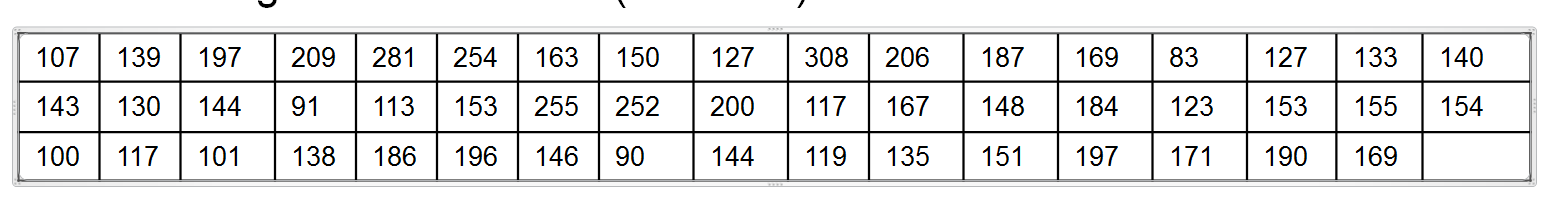
\includegraphics{Mcdonalds.png}

\hypertarget{relative-frequency-distribution}{%
\section{Relative Frequency Distribution}\label{relative-frequency-distribution}}

\begin{itemize}
\tightlist
\item
  Relative Frequency Distribution or Percentage Frequency Distribution: Each class frequency is replaced by a relative frequency (or proportion) or a percentage\\
  \[\textrm{Relative Frequency for a class}=\frac{\textrm{frequency for a class}}{\textrm{sum of all frequencies}}\]\\
\item
  Percentage Frequency: just convert the above to percent.
\item
  The sum of the percentages in a relative frequency distribution must be very close to 100\% (with a little wiggle room for rounding errors).
\end{itemize}

\hypertarget{cumulative-frequency-distribution}{%
\section{Cumulative Frequency Distribution}\label{cumulative-frequency-distribution}}

\begin{itemize}
\tightlist
\item
  \emph{Cumulative Frequency Distribution:} The frequency for each class is the sum of the frequencies for that class and all previous classes.
\end{itemize}

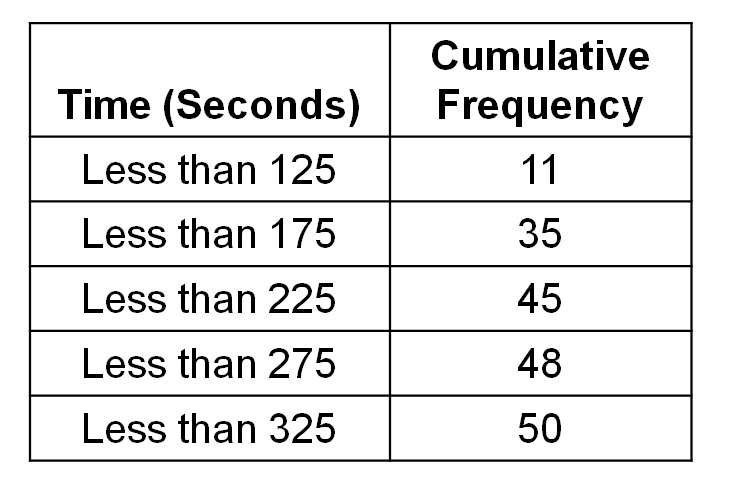
\includegraphics{Mcdonalds_cumul.png}

\hypertarget{cumulative-relative-frequence}{%
\section{Cumulative Relative Frequence}\label{cumulative-relative-frequence}}

\begin{itemize}
\tightlist
\item
  Simply divide the cumulative frequency by the total frequency.
\item
  If we plot the cumulative relative frequency, the plot is called the Ogive
\end{itemize}

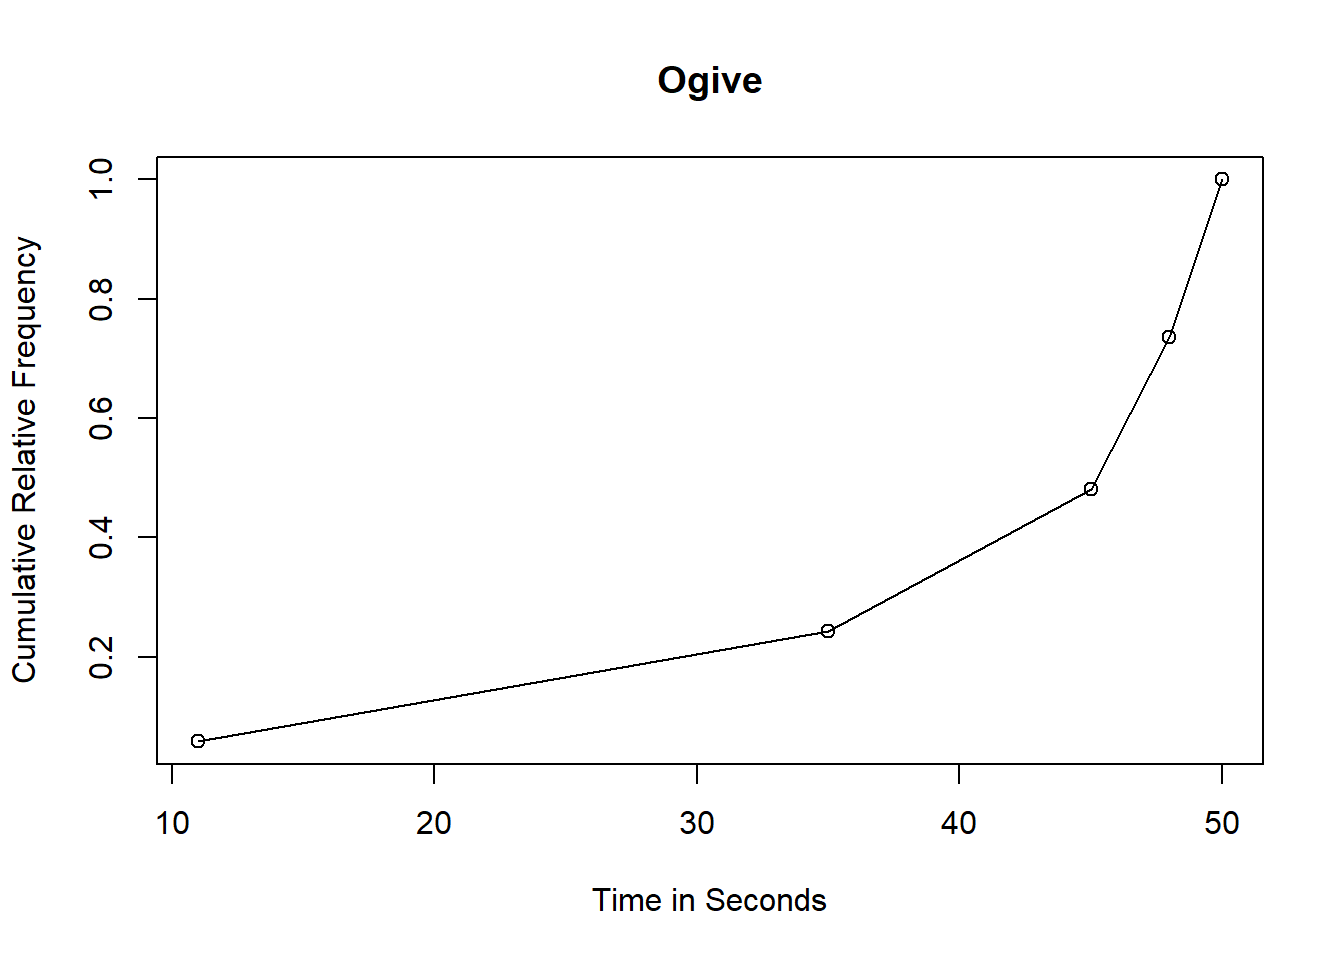
\includegraphics{Book_files/figure-latex/unnamed-chunk-7-1.pdf}

\hypertarget{using-frequency-distributions-to-understand-data}{%
\section{Using Frequency Distributions to Understand Data}\label{using-frequency-distributions-to-understand-data}}

We can roughly identify the distribution of a dataset using the frequency distribution. However, the more convinent way to do so is to use a historgram, which we will discuss later.

\hypertarget{gaps}{%
\section{Gaps}\label{gaps}}

\begin{itemize}
\tightlist
\item
  The presence of gaps can show that the data are from two or more different populations.
\item
  However, the converse is not true, because data from different populations do not necessarily result in gaps.
\end{itemize}

\hypertarget{what-do-gaps-tell-us}{%
\section{What Do Gaps Tell Us?}\label{what-do-gaps-tell-us}}

The table shown is a frequency distribution of the weights (grams) of randomly selected pennies.\\
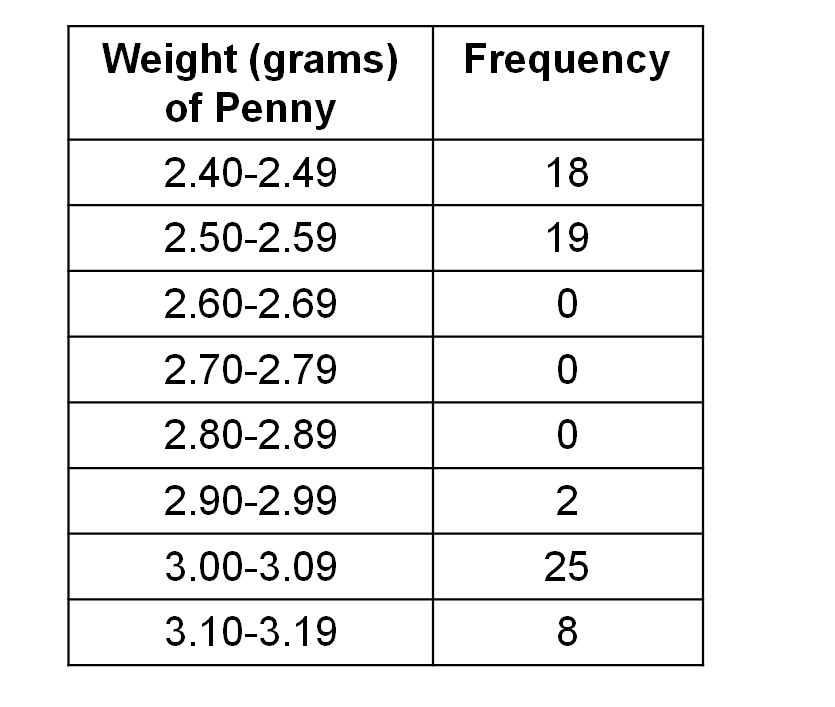
\includegraphics{gap.png}

\begin{itemize}
\tightlist
\item
  Pennies made before 1983 are 95\% copper and 5\% zinc.
\item
  Pennies made after 1983 are 2.5\% copper and 97.5\% zinc.
\end{itemize}

\hypertarget{histogram}{%
\section{Histogram}\label{histogram}}

\begin{itemize}
\tightlist
\item
  \textbf{Histogram:} A graph consisting of bars of equal width drawn adjacent to each other (unless there are gaps in the data). The horizontal scale represents classes of quantitative data values, and the vertical scale represents frequencies. The heights of the bars correspond to frequency values.
\end{itemize}

\hypertarget{important-uses-of-a-histogram}{%
\section{Important Uses of a Histogram}\label{important-uses-of-a-histogram}}

\begin{itemize}
\tightlist
\item
  Visually displays the shape of the distribution of the data
\item
  Shows the location of the center of the data
\item
  Shows the spread of the data
\item
  Identifies outliers
\end{itemize}

\hypertarget{example-of-a-histogram}{%
\section{Example of A Histogram}\label{example-of-a-histogram}}

\begin{itemize}
\tightlist
\item
  \emph{Relative Frequency Histogram:} It has the same shape and horizontal scale as a histogram, but the vertical scale is marked with relative frequencies instead of actual frequencies.
  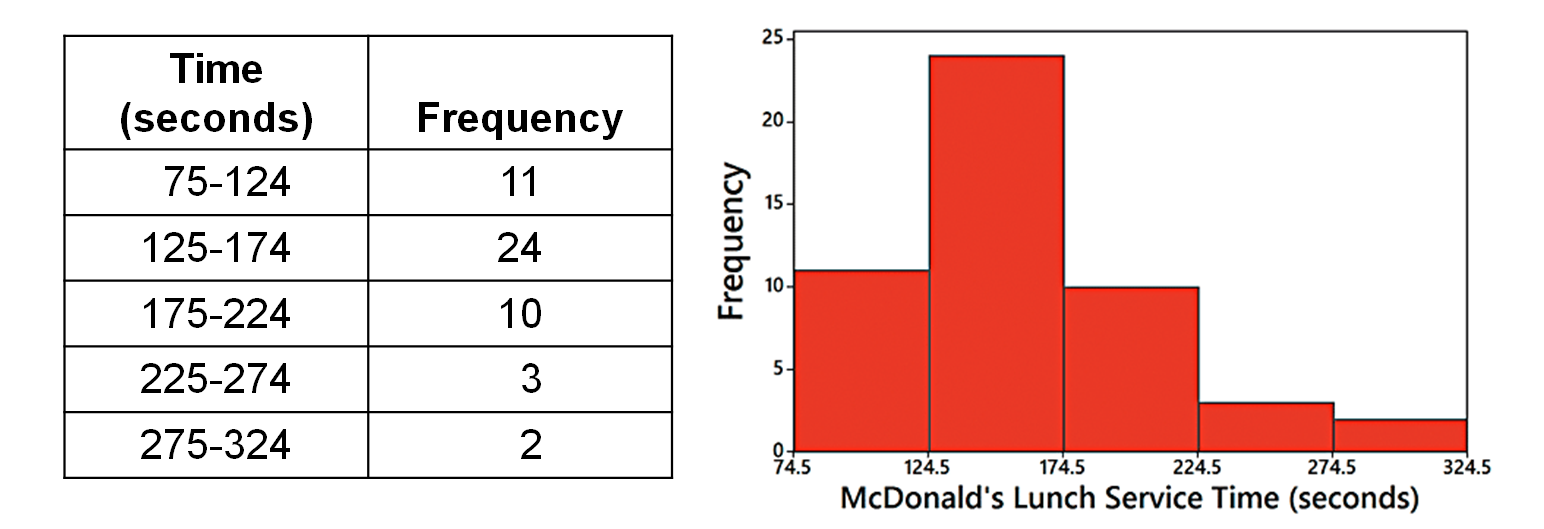
\includegraphics{histogram.png}
\end{itemize}

\hypertarget{interpreting-histograms}{%
\section{Interpreting Histograms}\label{interpreting-histograms}}

\begin{itemize}
\item
  Explore the data by analyzing the histogram to see what can be learned about ``CVDOT'':

  \begin{itemize}
  \tightlist
  \item
    the Center of the data,
  \item
    the Variation,
  \item
    the shape of the Distribution,
  \item
    whether there are any Outliers,
  \item
    and Time. (if possible)
  \end{itemize}
\end{itemize}

\hypertarget{common-distribution-shapes}{%
\section{Common Distribution Shapes}\label{common-distribution-shapes}}

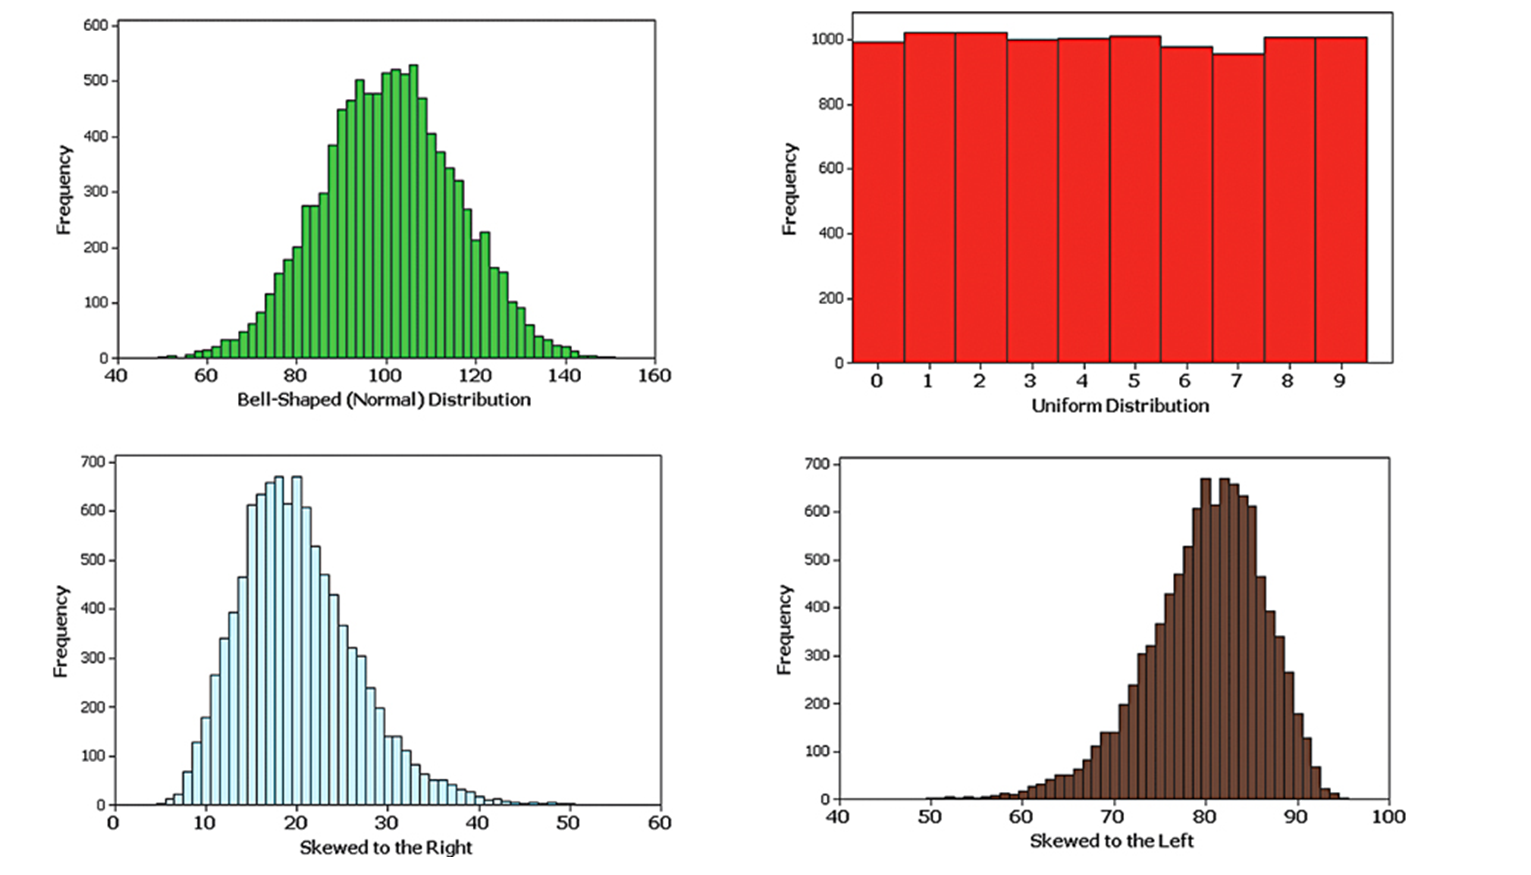
\includegraphics{shapes.png}

\hypertarget{assessing-normality-with-normal-quantile-plots-q-q-plots}{%
\section{Assessing Normality with Normal Quantile Plots (Q-Q plots)}\label{assessing-normality-with-normal-quantile-plots-q-q-plots}}

\begin{itemize}
\tightlist
\item
  Criteria for Assessing Normality with a Normal Quantile Plot

  \begin{itemize}
  \tightlist
  \item
    Normal Distribution: The pattern of the points in the normal quantile plot is reasonably close to a straight line, and the points do not show some systematic pattern that is not a straight-line pattern.
  \item
    Not a Normal Distribution: The population distribution is not normal if the normal quantile plot has either or both of these two conditions:

    \begin{itemize}
    \tightlist
    \item
      The points do not lie reasonably close to a straight-line pattern.
    \item
      The points show some systematic pattern that is not a straight-line pattern. (going up and down around the line)
    \end{itemize}
  \end{itemize}
\end{itemize}

\hypertarget{examples-of-q-q-plots}{%
\section{Examples of Q-Q plots}\label{examples-of-q-q-plots}}

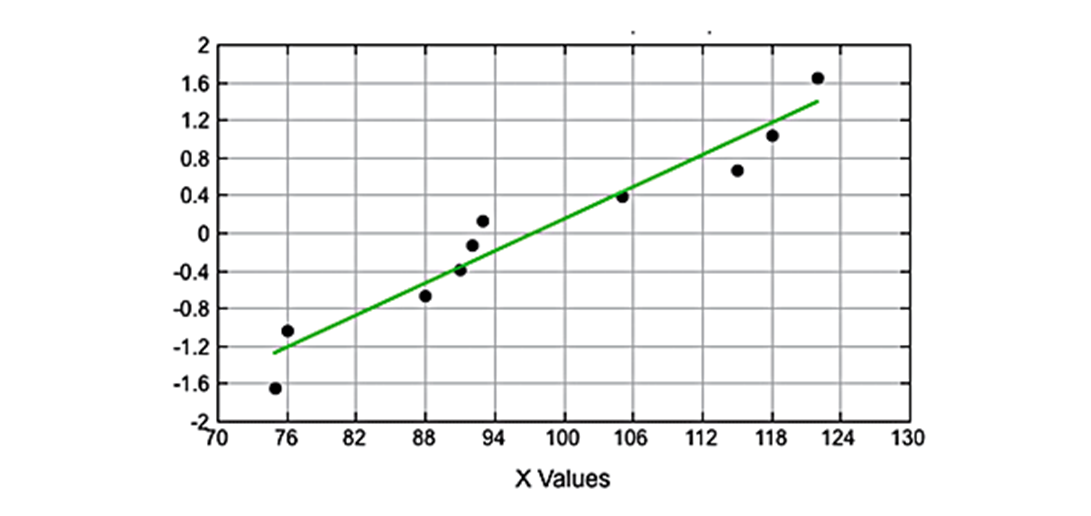
\includegraphics{normal_QQ.png}

Normal Distribution: The points are reasonably close to a straight-line pattern, and there is no other systematic pattern that is not a straight-line pattern.

\begin{center}\rule{0.5\linewidth}{\linethickness}\end{center}

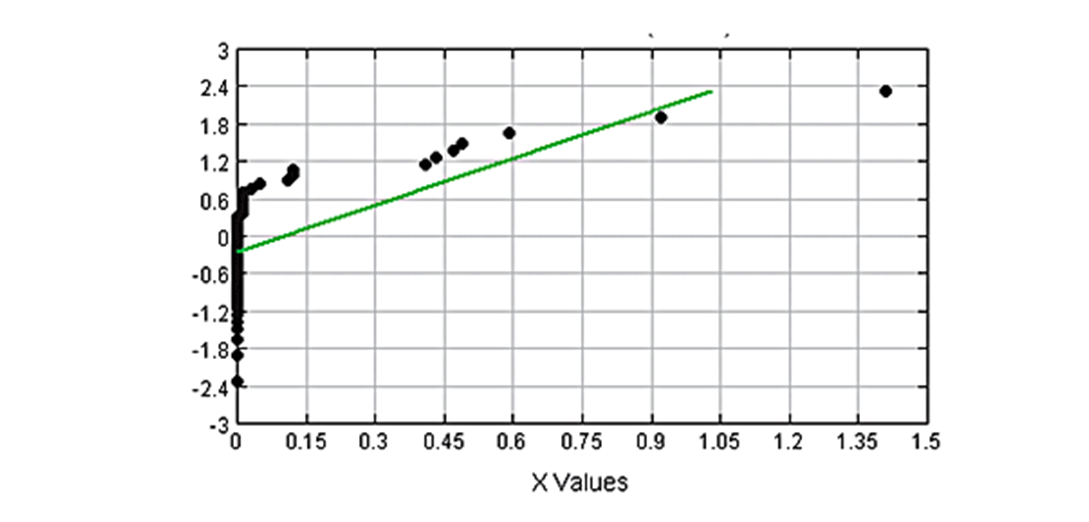
\includegraphics{not_normal_QQ_1.png}

Not a Normal Distribution: The points do not lie reasonably close to a straight line.

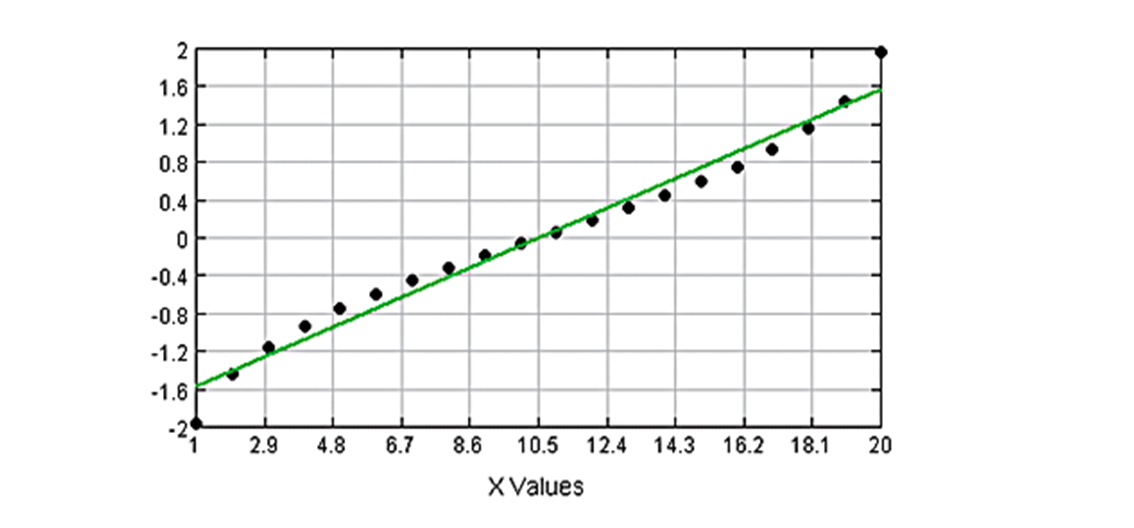
\includegraphics{not_normal_QQ_2.png}

Not a Normal Distribution: The points show a systematic pattern that is not a straight-line pattern.

\hypertarget{dotplots}{%
\section{Dotplots}\label{dotplots}}

\begin{itemize}
\tightlist
\item
  A graph of quantitative data in which each data value is plotted as a point (or dot) above a horizontal scale of values. Dots representing equal values are stacked.
\end{itemize}

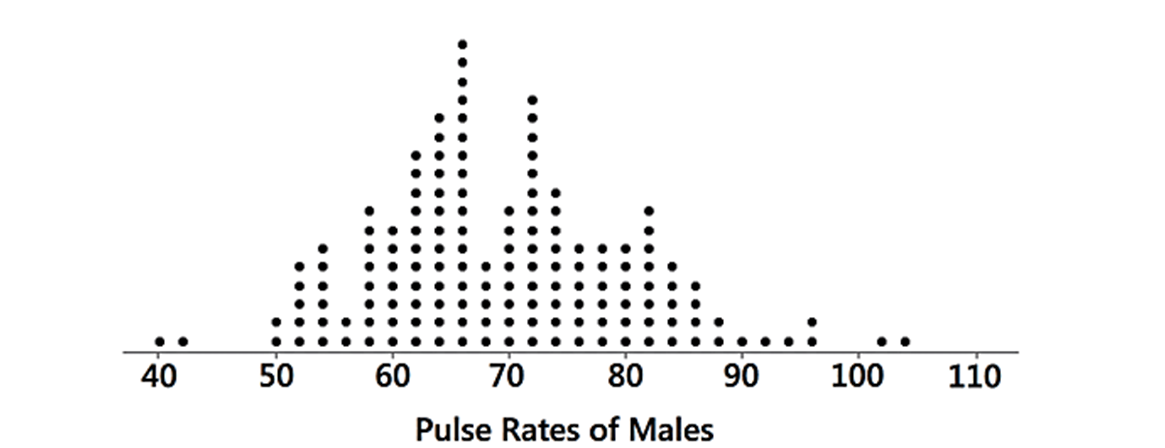
\includegraphics{dot.png}

\begin{itemize}
\tightlist
\item
  Features of a Dotplot

  \begin{itemize}
  \tightlist
  \item
    Displays the shape of distribution of data.
  \item
    It is usually possible to recreate the original list of data values.
  \end{itemize}
\end{itemize}

\hypertarget{stemplots-you-need-to-assign-a-key-to-read-a-stem-plot}{%
\section{Stemplots (You need to assign a key to read a stem plot)}\label{stemplots-you-need-to-assign-a-key-to-read-a-stem-plot}}

Represents quantitative data by separating each value into two parts: the stem (such as the leftmost digit) and the leaf (such as the rightmost digit).
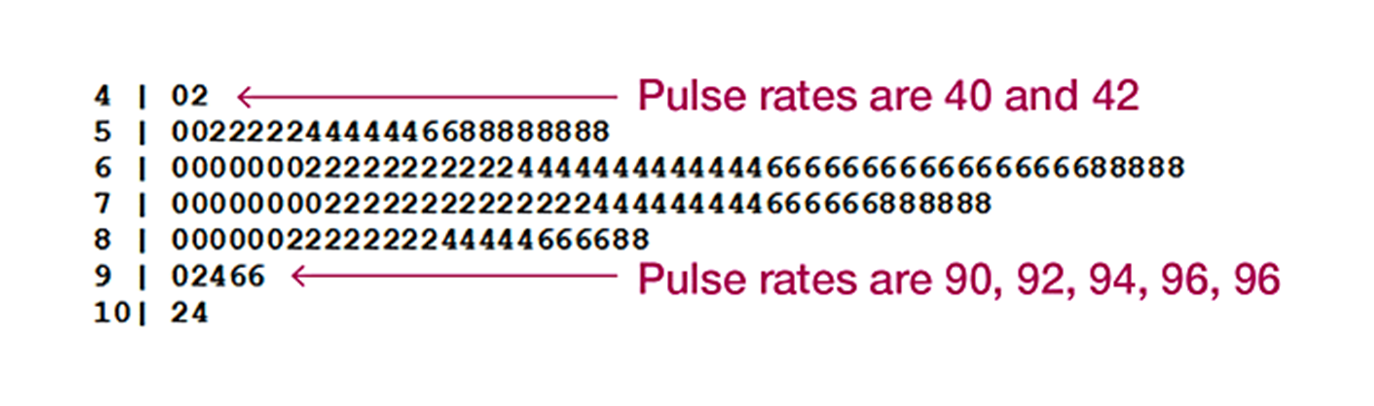
\includegraphics{stem.png}

\begin{itemize}
\tightlist
\item
  Features of a Stemplot

  \begin{itemize}
  \tightlist
  \item
    Shows the shape of the distribution of the data.
  \item
    Retains the original data values.
  \item
    The sample data are sorted (arranged in order).
  \end{itemize}
\end{itemize}

\hypertarget{bar-graph}{%
\section{Bar Graph}\label{bar-graph}}

Shows the relative distribution of categorical data so that it is easier to compare the different categories.

\hypertarget{pareto-chart}{%
\section{Pareto Chart}\label{pareto-chart}}

A Pareto chart is a bar graph for categorical data, with the added stipulation that the bars are arranged in descending order according to frequencies, so the bars decrease in height from left to right.

\begin{itemize}
\tightlist
\item
  Features of a Pareto Chart

  \begin{itemize}
  \tightlist
  \item
    Shows the relative distribution of categorical data so that it is easier to compare the different categories.
  \item
    Draws attention to the more important categories.
  \end{itemize}
\end{itemize}

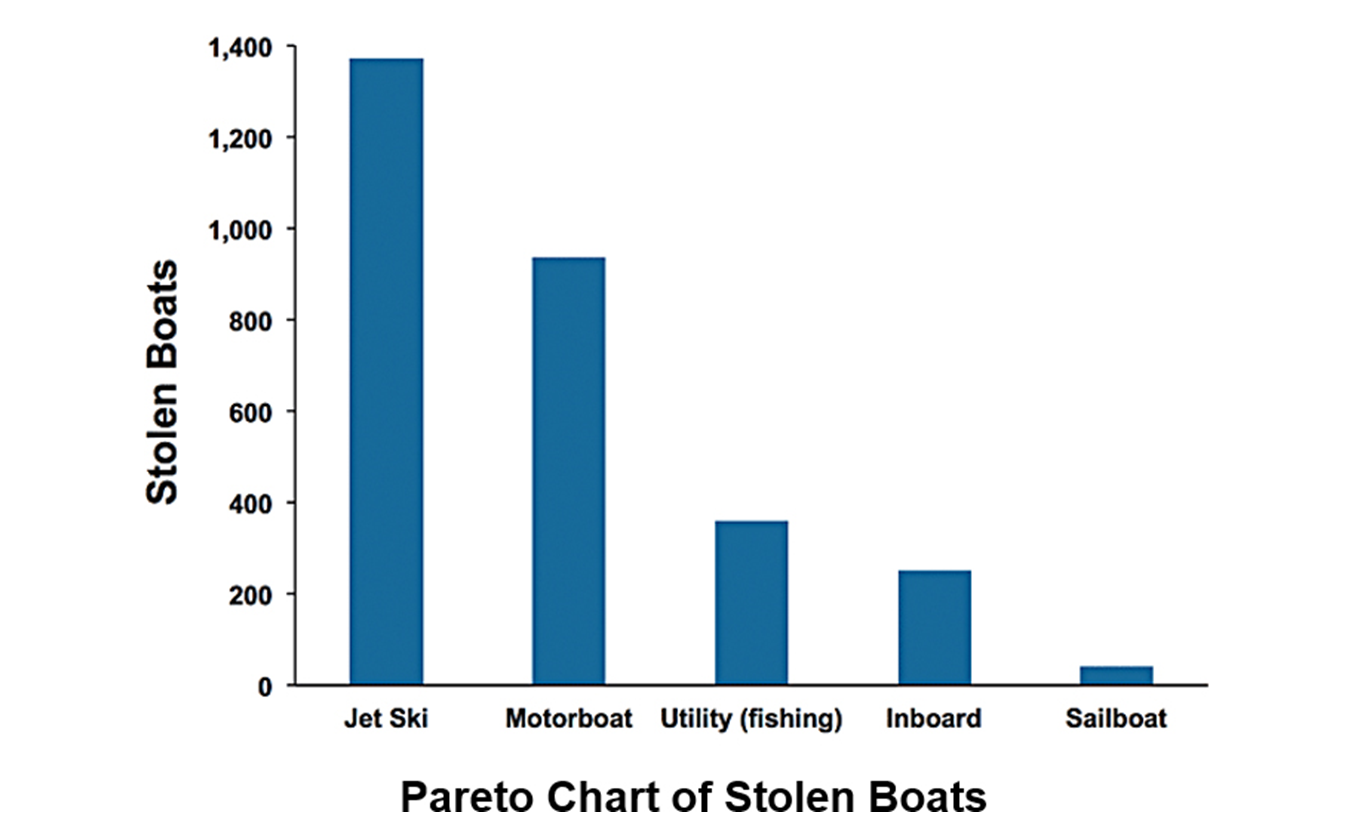
\includegraphics{pareto.png}

\hypertarget{pie-charts}{%
\section{Pie Charts}\label{pie-charts}}

A very common graph that depicts categorical data as slices of a circle, in which the size of each slice is proportional to the frequency count for the category; Shows the distribution of categorical data in a commonly used format.
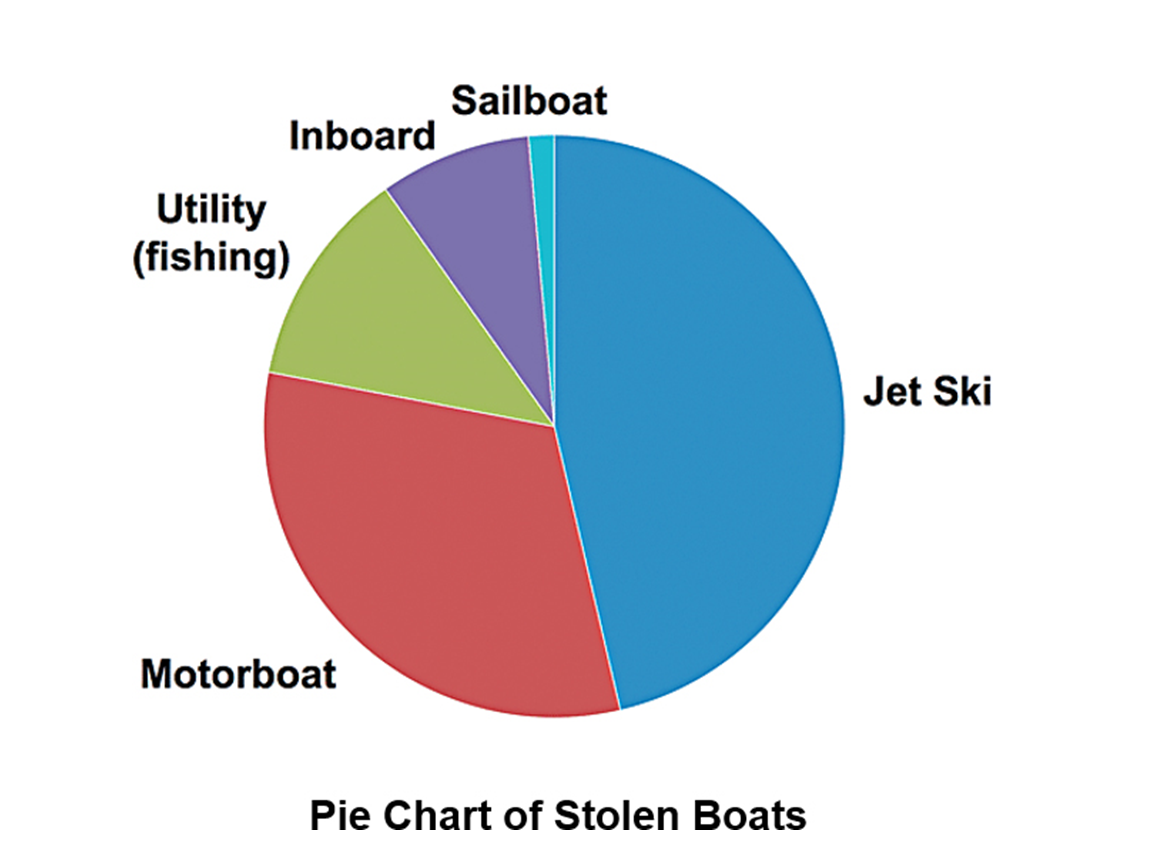
\includegraphics{pie.png}

\hypertarget{frequency-polygon}{%
\section{Frequency Polygon}\label{frequency-polygon}}

\begin{itemize}
\tightlist
\item
  A graph using line segments connected to points located directly above class midpoint values
\item
  A frequency polygon is very similar to a histogram, but a frequency polygon uses line segments instead of bars.
  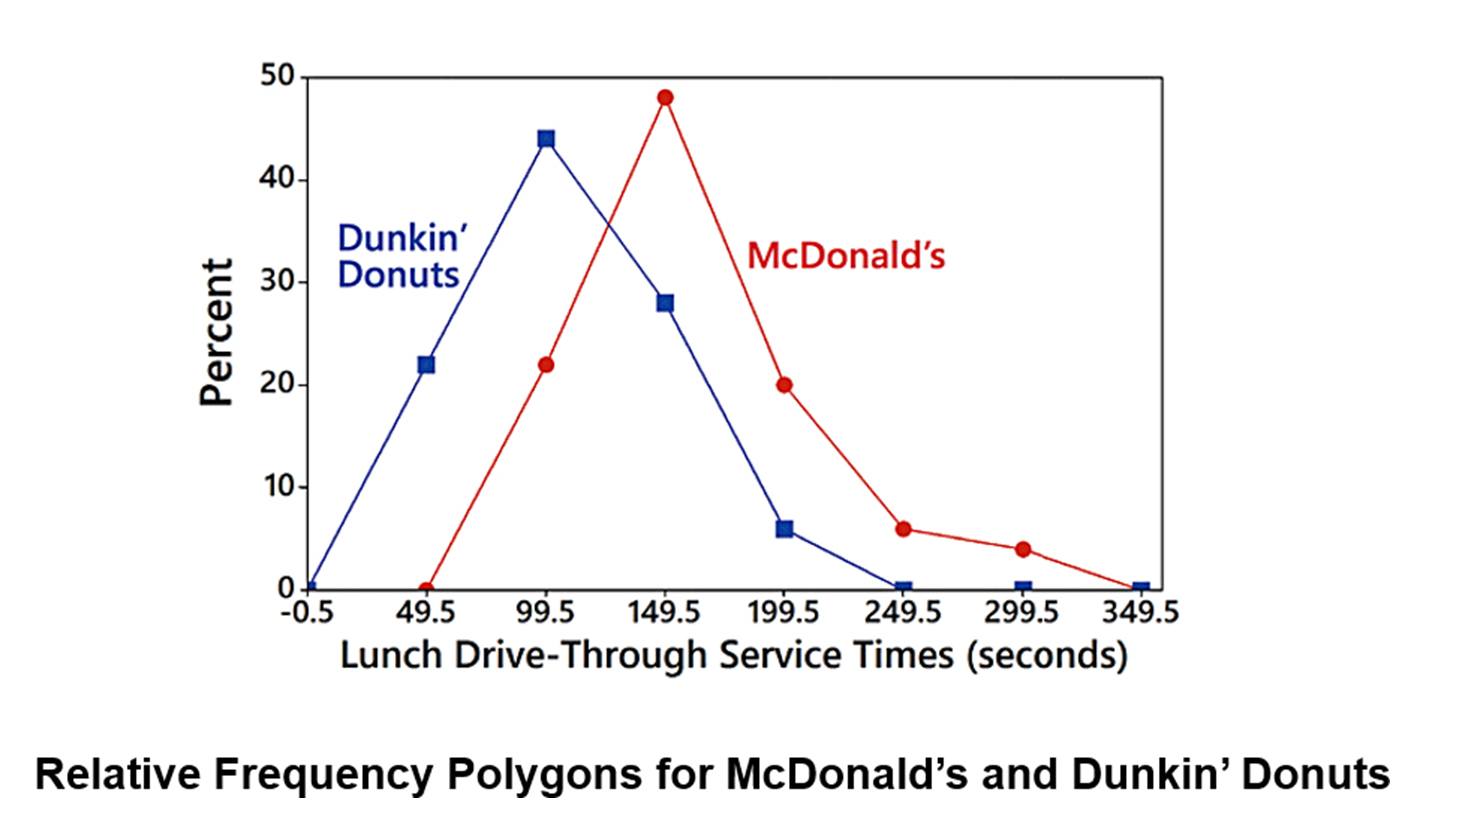
\includegraphics{polygon.png}
\end{itemize}

\hypertarget{graphs-that-deceive}{%
\section{Graphs That Deceive}\label{graphs-that-deceive}}

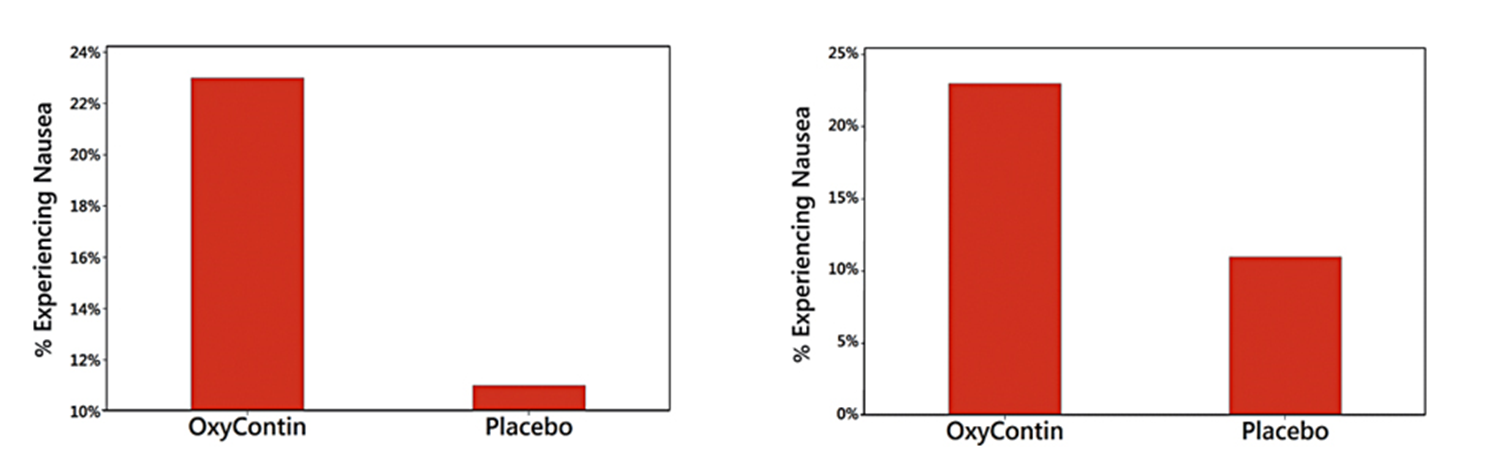
\includegraphics{wrong_graph_1.png}

\hypertarget{pictographs}{%
\section{Pictographs}\label{pictographs}}

\begin{itemize}
\tightlist
\item
  By using pictographs, artists can create false impressions that grossly distort differences by using these simple principles of basic geometry:

  \begin{itemize}
  \tightlist
  \item
    When you double each side of a square, its area doesn't merely double; it increases by a factor of four.
  \item
    When you double each side of a cube, its volume doesn't merely double; it increases by a factor of eight.
    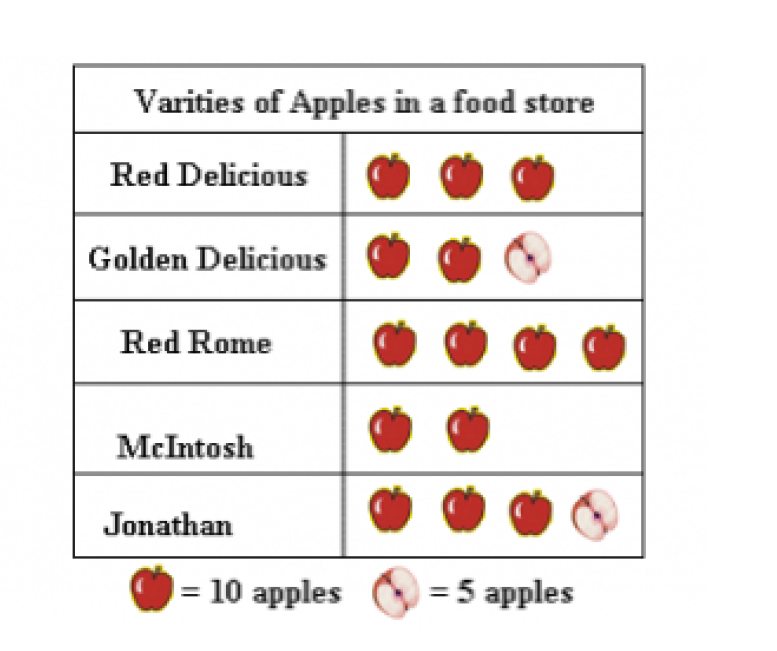
\includegraphics{picto.png}
  \end{itemize}
\end{itemize}

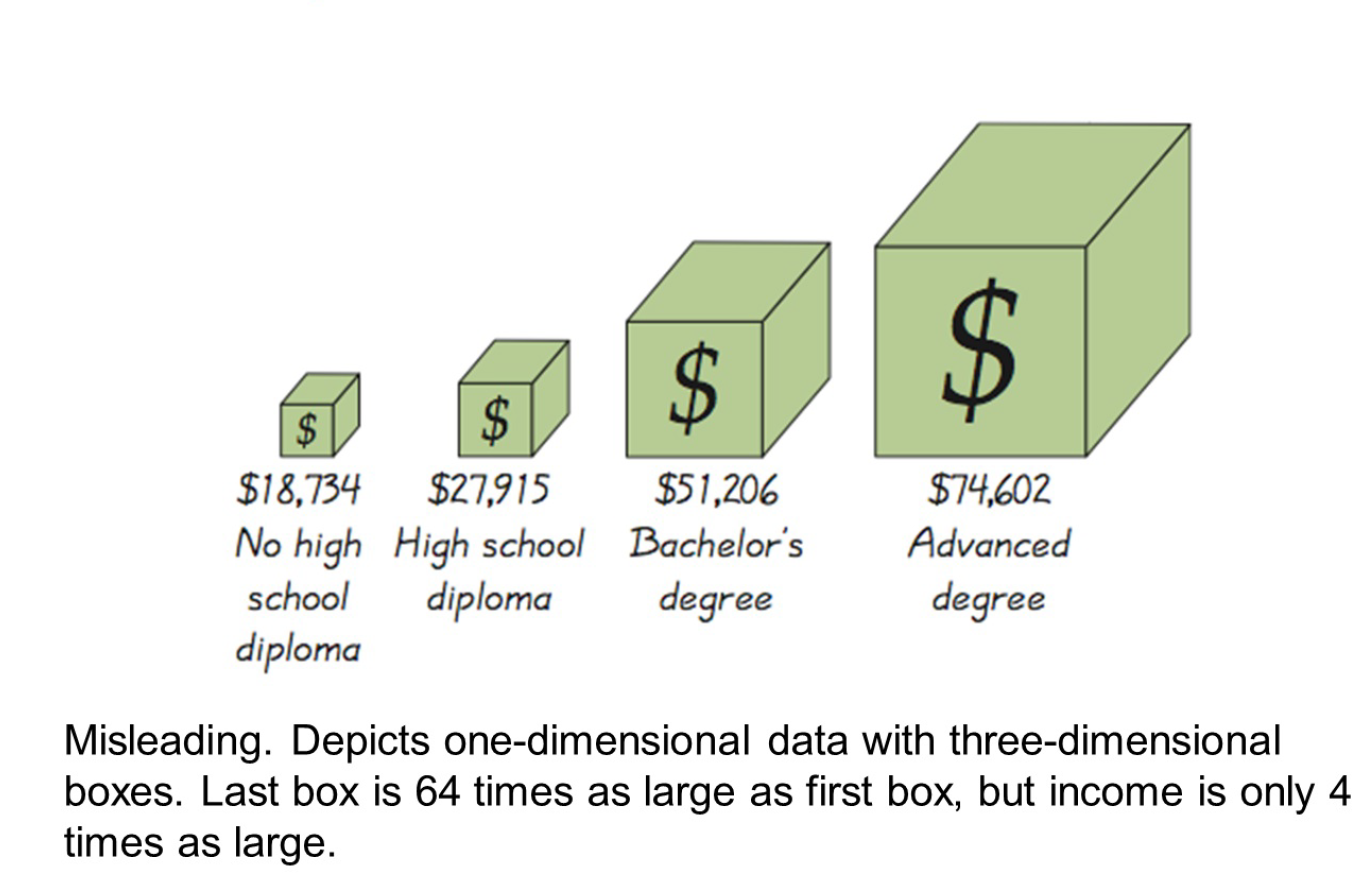
\includegraphics{picto_wrong.png}

\hypertarget{scatterplot-two-numerical-variables}{%
\section{Scatterplot (Two Numerical Variables)}\label{scatterplot-two-numerical-variables}}

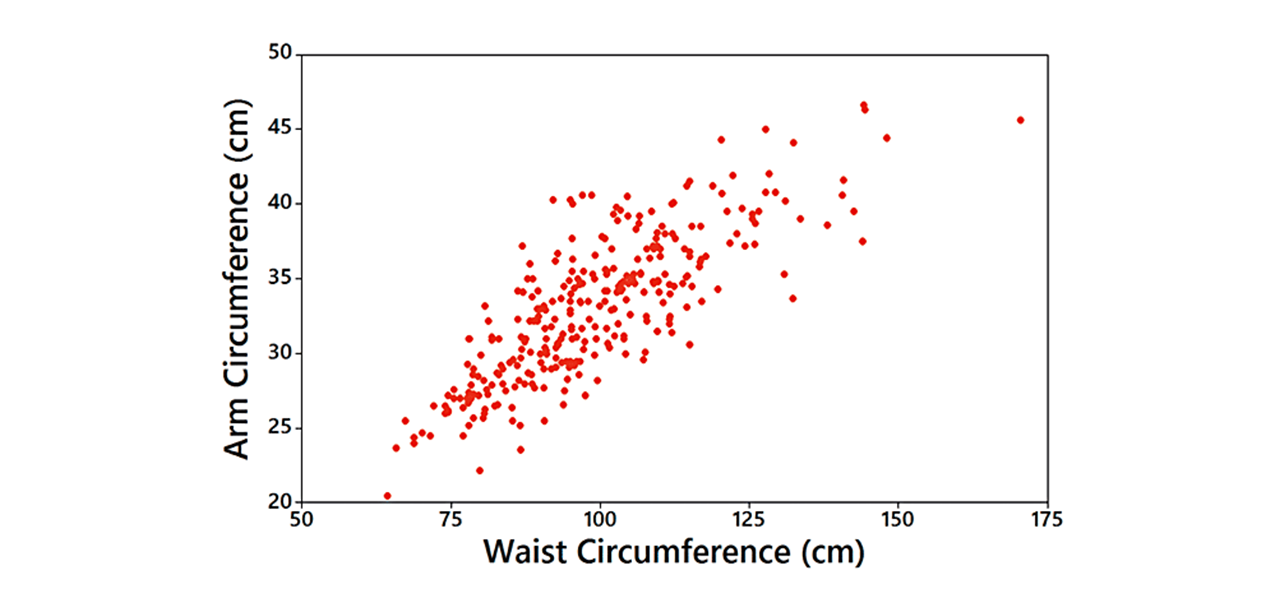
\includegraphics{scatter.png}

\hypertarget{nba}{%
\section{NBA}\label{nba}}

\begin{itemize}
\tightlist
\item
  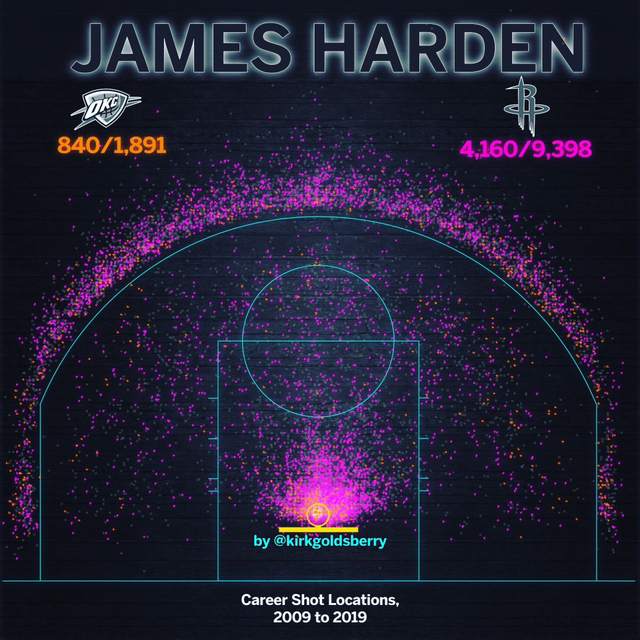
\includegraphics{James_Harden.jpg}
\item
  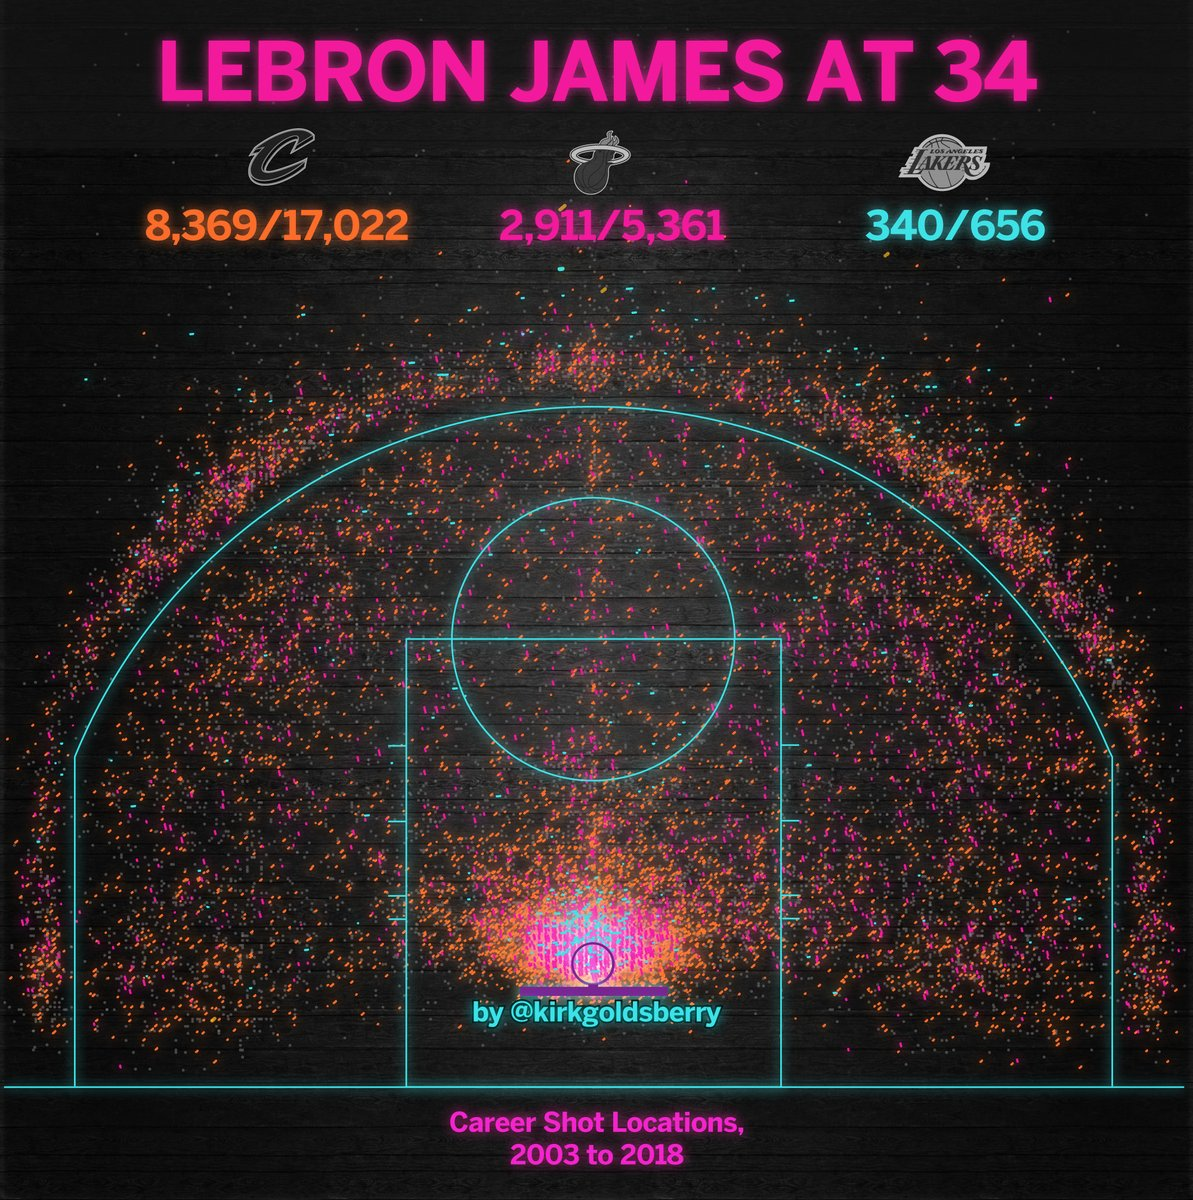
\includegraphics{Lebron_James.jpg}
\item
  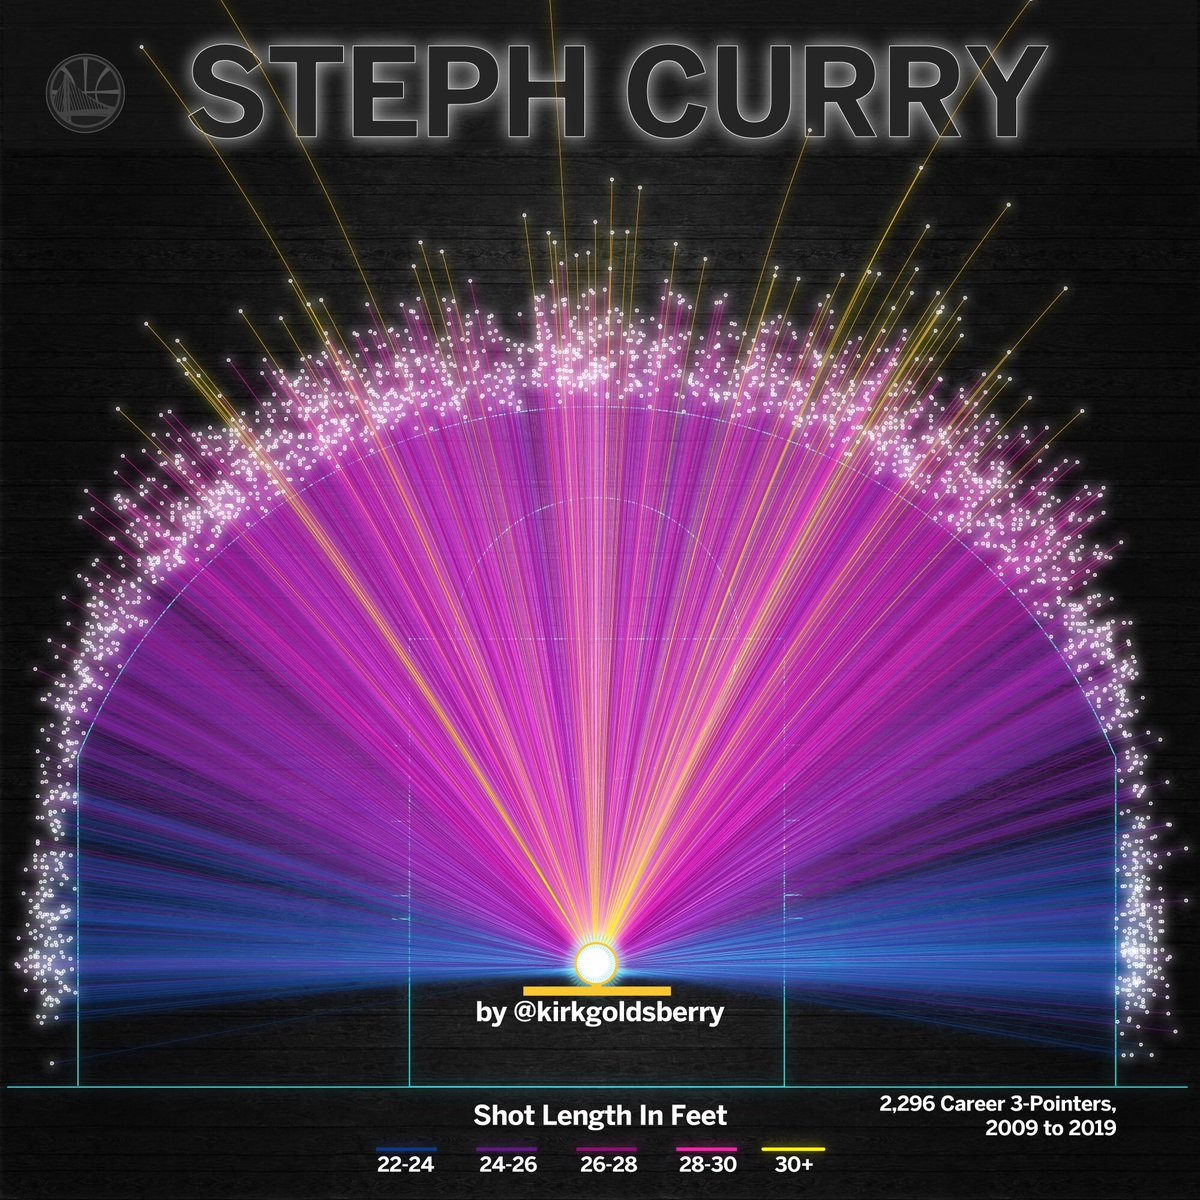
\includegraphics{Steph_Curry.jpg}
\end{itemize}

\hypertarget{descriptive-statistics}{%
\chapter{Descriptive Statistics}\label{descriptive-statistics}}

\begin{itemize}
\item
  In this chapter we'll learn to summarize or describe the important characteristics of a data set (mean, standard
  deviation, etc.)
\item
  The focus of this section is to obtain a value that measures the center of a data set. In particular, we present measures of center, including mean and median. Our objective here is not only to find the value of each measure of center, but also to interpret those values.
\item
  A measure of center is a value at the center or middle of a data set.
\end{itemize}

\hypertarget{mean-or-arithmetic-mean}{%
\section{Mean (or Arithmetic Mean)}\label{mean-or-arithmetic-mean}}

\begin{itemize}
\tightlist
\item
  The \textbf{mean (or arithmetic mean)} of a set of data is the measure of center found by adding all of the data values and dividing the total by the number of data values.
  \[\bar{x}=\frac{\sum x_i}{n}\]
\item
  Sample means drawn from the same population tend to vary less than other measures of center.
\item
  The mean of a data set uses every data value.
\item
  A disadvantage of the mean is that just one extreme value (outlier) can change the value of the mean substantially. (Using the following definition, we say that the mean is not \textbf{resistant}.)
\item
  A statistic is resistant if the presence of extreme values (outliers) does not cause it to change very much.
\item
  Caution: We don't use the term average in Statistics. Instead, we use the term mean, or expected value, which will be introduced later.
\end{itemize}

\hypertarget{notations}{%
\section{Notations}\label{notations}}

\begin{itemize}
\tightlist
\item
  \(\sum\) denotes the sum of a set of values.
\item
  \(x\) is the variable usually used to represent the individual data values.
\item
  \(n\) represents the number of data values in a sample.
\item
  \(N\) represents the number of data values in a population.
\item
  \(\bar{x}\): the mean of a set of sample values (sample mean)
\item
  \(\bar{x}=\frac{\sum{x}}{n}\)
\item
  \(\mu\): the mean of all values in a population (population mean)
\item
  \(\mu=\frac{\sum{x}}{N}\)
\end{itemize}

\hypertarget{mean-example}{%
\section{Mean-Example}\label{mean-example}}

\begin{itemize}
\item
  Find the mean of the first five data speeds for Verizon: 38.5, 55.6, 22.4, 14.1, and 23.1 (all in megabits per second, or Mbps).
\item
  Find the mean of the first five counts for Chips Ahoy regular cookies: 22 chips, 22 chips, 26 chips, 24 chips, and 23 chips.
\end{itemize}

\hypertarget{median}{%
\section{Median}\label{median}}

\begin{itemize}
\tightlist
\item
  Median is the middle value when the original data values are arranged in order of increasing (or decreasing) magnitude
\item
  often denoted by \(\tilde{x}\)\\
\item
  is not affected by an extreme value - is a resistant measure of the center
\item
  To find the median, first sort the values (arrange them in order) and then follow one of these two procedures:

  \begin{itemize}
  \tightlist
  \item
    If the number of data values is odd, the median is the number located in the exact middle of the sorted list.
  \item
    If the number of data values is even, the median is found by computing the mean of the two middle numbers in the sorted list.
  \end{itemize}
\end{itemize}

\hypertarget{median-example}{%
\section{Median-Example}\label{median-example}}

\begin{itemize}
\tightlist
\item
  Find the median of the first five data speeds for Verizon: 38.5, 55.6, 22.4, 14.1, and 23.1 (all in megabits per second, or Mbps).
\item
  Repeat of the previous example after including the sixth data speed of 24.5 Mbps. That is, find the median of these data speeds: 38.5, 55.6, 22.4, 14.1, 23.1, 24.5 (all in Mbps).
\end{itemize}

\hypertarget{which-one-do-you-use-mean-or-median}{%
\section{Which one do you use? Mean or Median?}\label{which-one-do-you-use-mean-or-median}}

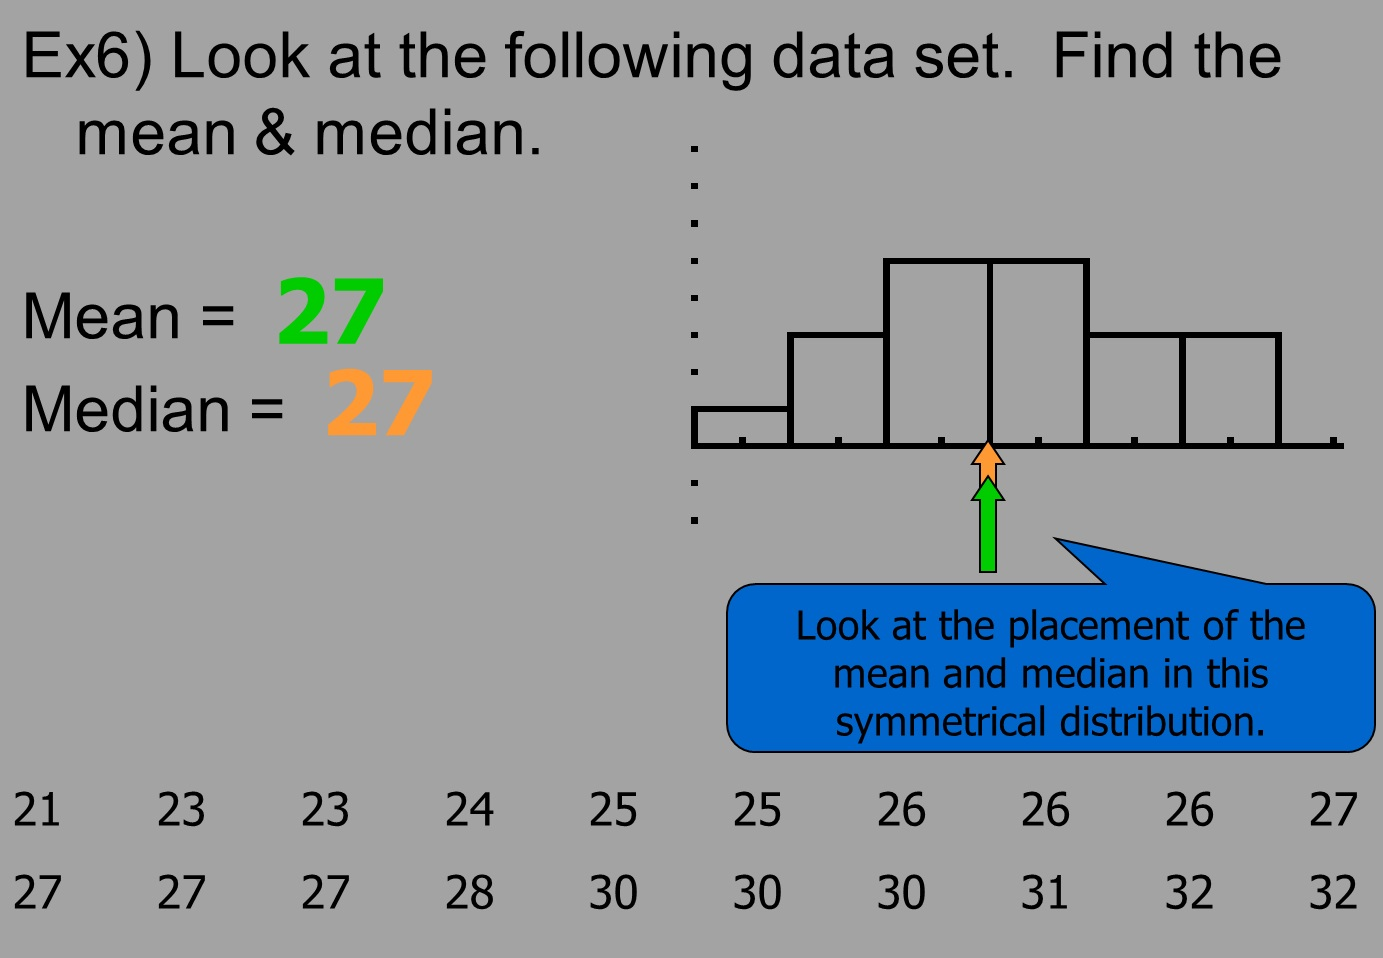
\includegraphics{pic5.jpg}

\begin{center}\rule{0.5\linewidth}{\linethickness}\end{center}

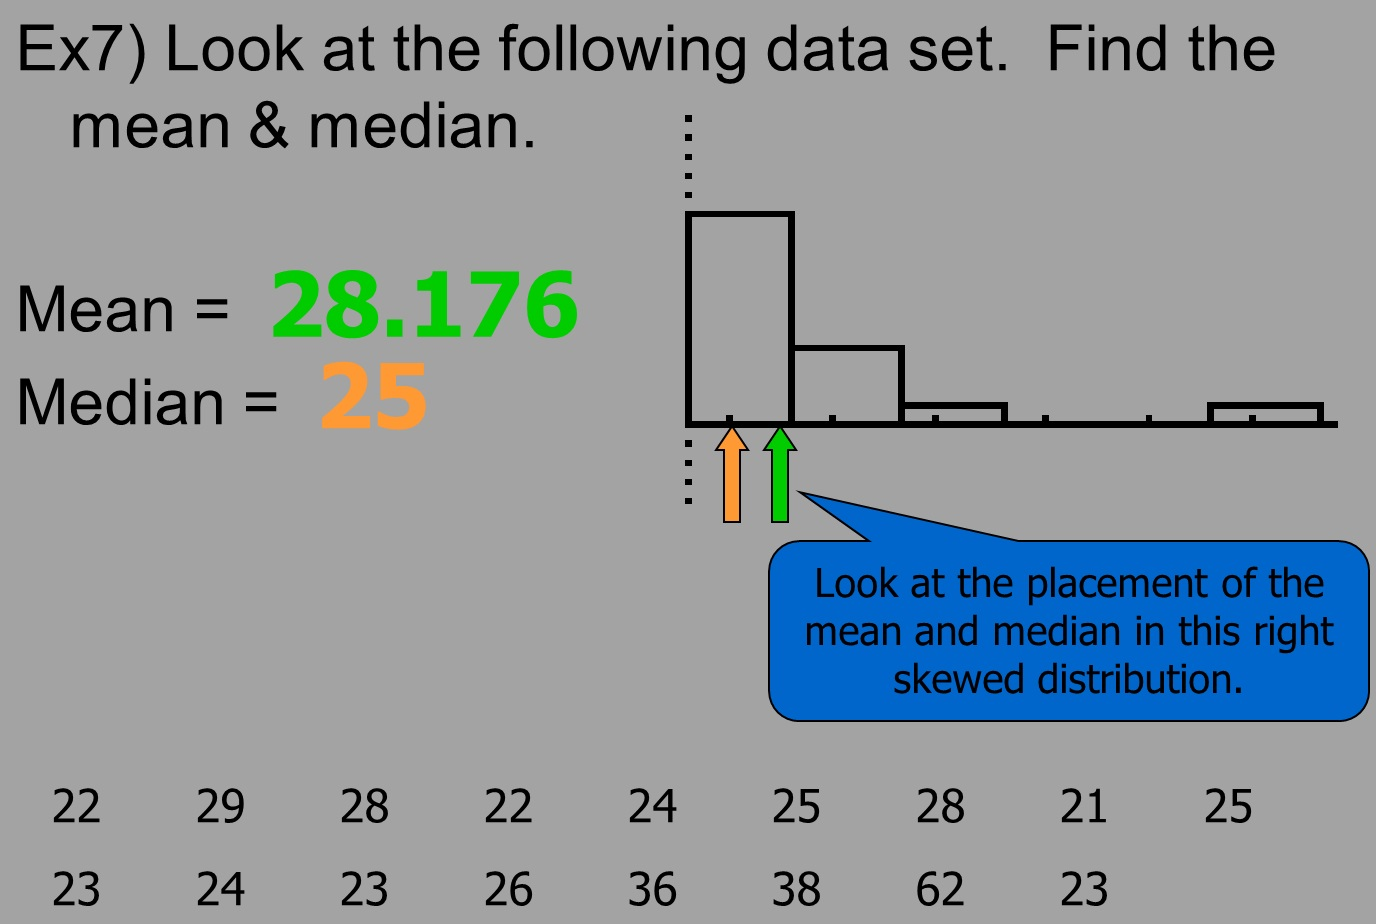
\includegraphics{pic6.jpg}

\begin{center}\rule{0.5\linewidth}{\linethickness}\end{center}

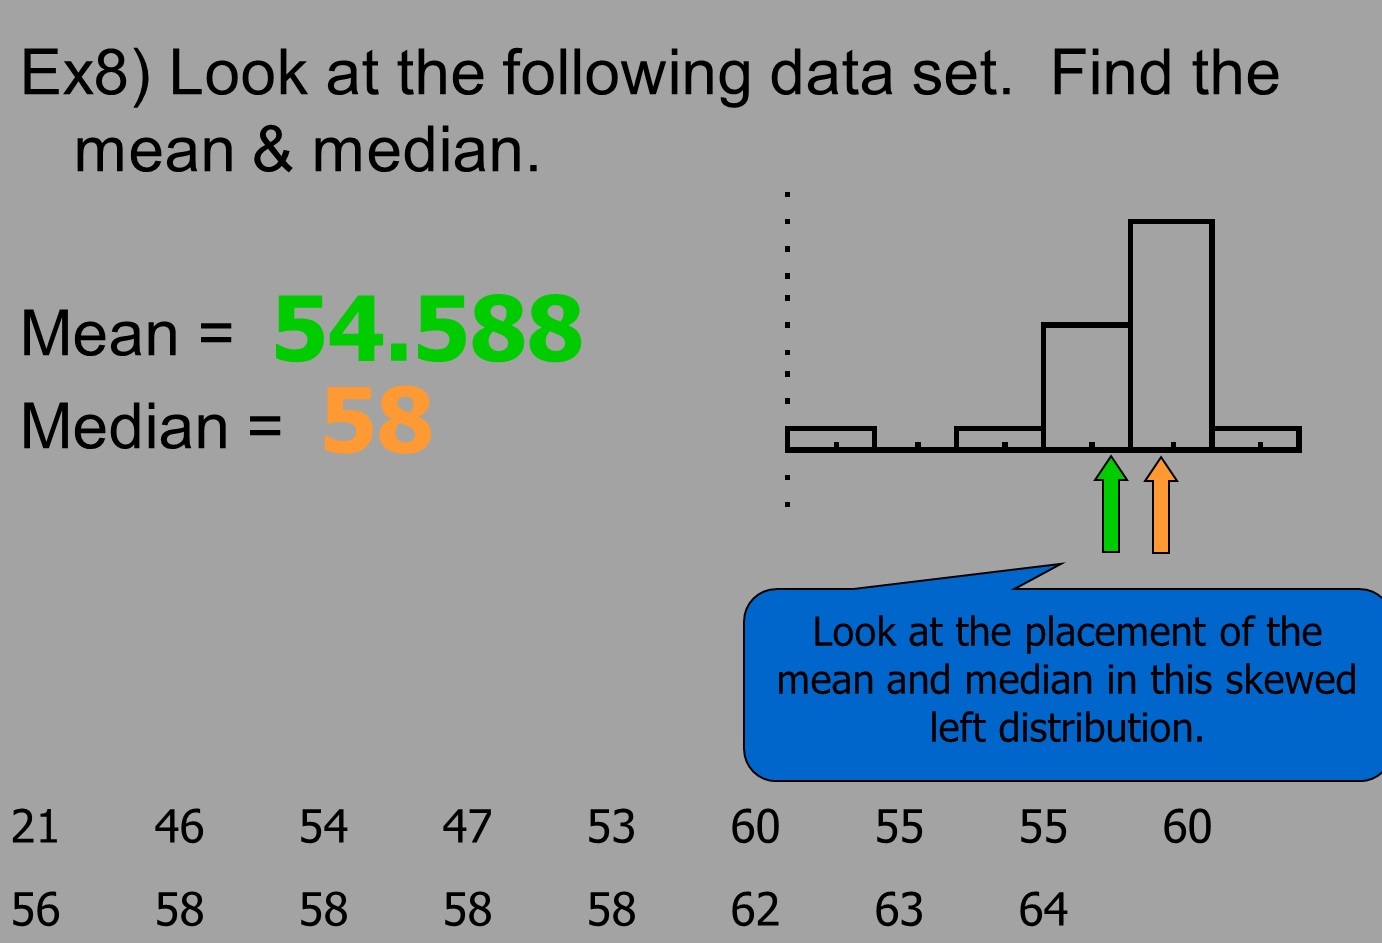
\includegraphics{pic7.jpg}

\hypertarget{which-one-do-you-use-mean-or-median-1}{%
\section{Which one do you use? Mean or Median?}\label{which-one-do-you-use-mean-or-median-1}}

\begin{itemize}
\tightlist
\item
  In a symmetrical distribution, the mean and median are equal.
\item
  In a skewed distribution, the mean is pulled in the direction of the skewness.
\item
  In a symmetrical distribution, you should report the mean!
\item
  In a skewed distribution, the median should be reported as the measure of center!
\end{itemize}

\hypertarget{mode}{%
\section{Mode}\label{mode}}

\begin{itemize}
\tightlist
\item
  Mode is the value that occurs with the greatest frequency
\item
  Data set can have one, more than one, or no mode
\item
  Bimodal two data values occur with the same greatest frequency
\item
  Multimodal more than two data values occur with the same greatest frequency
\item
  No Mode no data value is repeated
\item
  Mode is the only measure of central tendency that can be used with \textbf{nominal} data.
\end{itemize}

\hypertarget{mode-example}{%
\section{Mode-Example}\label{mode-example}}

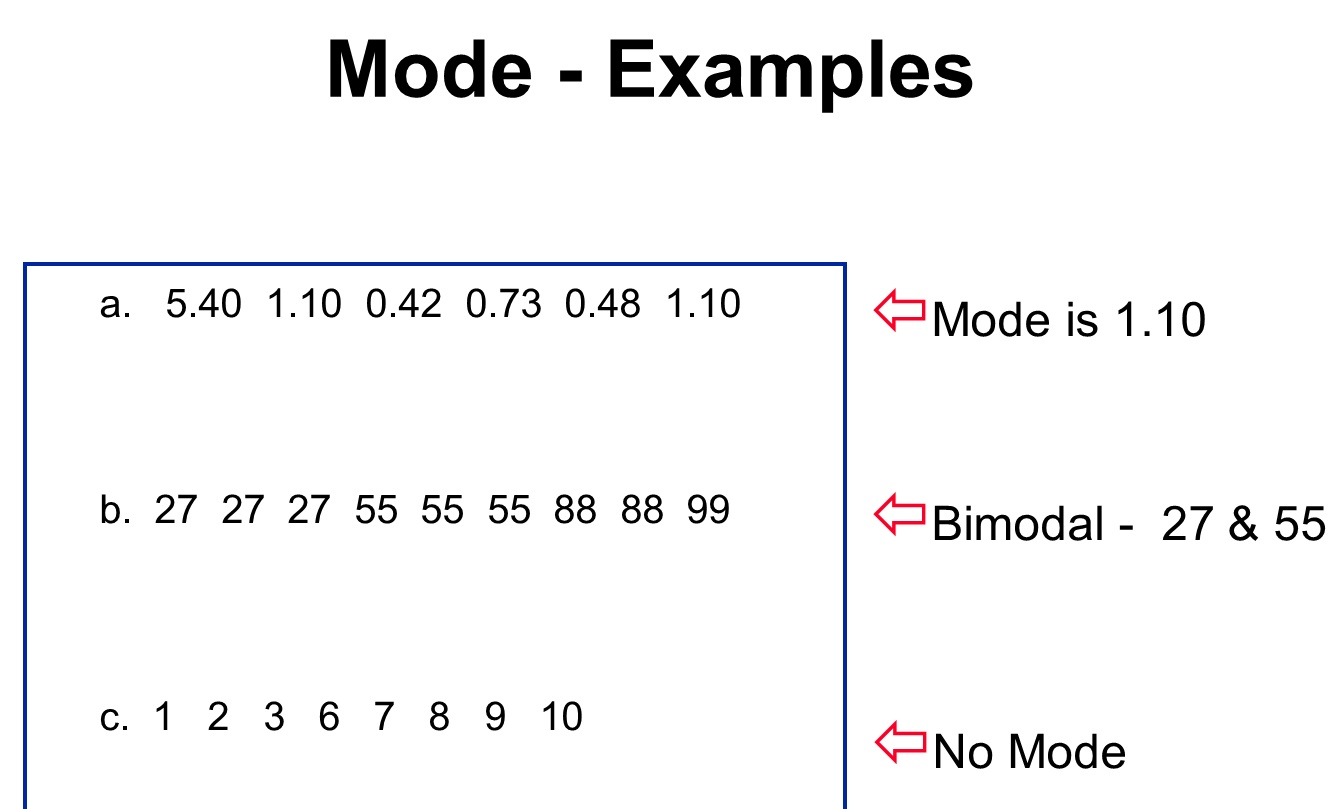
\includegraphics{pic8.jpg}

\hypertarget{midrange}{%
\section{Midrange}\label{midrange}}

\begin{itemize}
\tightlist
\item
  Midrange is the value midway between the maximum and minimum values in the original data set
\item
  \(Midrange=\frac{Maximum \enspace Value +Minimum \enspace Value}{2}\)
\item
  Because the midrange uses only the maximum and minimum values, it is very sensitive to those extremes so the midrange is not resistant.
\end{itemize}

\hypertarget{round-off-rules-for-measures-of-center}{%
\section{Round-Off Rules for Measures of Center}\label{round-off-rules-for-measures-of-center}}

\begin{itemize}
\tightlist
\item
  For the mean, median, and midrange, carry one more decimal place than is present in the original set of values.
\item
  For the mode, leave the value as is without rounding (because values of the mode are the same as some of the original data values).
\end{itemize}

\hypertarget{calculating-a-weighted-mean}{%
\section{Calculating a Weighted Mean}\label{calculating-a-weighted-mean}}

\begin{itemize}
\tightlist
\item
  When data values are assigned different weights, \(w\), we can compute a weighted mean.
  \[\bar{x}=\frac{\sum{(w\cdot x)}}{\sum{w}}\]
\item
  In her first semester of college, a student of the author took five courses.
  Her final grades along with the number of credits for each course were A (3 credits), A (4 credits), B (3 credits), C (3 credits), and F (1 credit).
  The grading system assigns quality points to letter grades as follows:
  A = 4; B = 3; C = 2; D = 1; F = 0.
\end{itemize}

\hypertarget{more-examples-about-finding-the-means}{%
\section{More Examples About Finding The Means}\label{more-examples-about-finding-the-means}}

\begin{itemize}
\tightlist
\item
  Angelique made scores of 85, 56, and 91 on her first three statistic tests. What does she need to make on her next test to have an 80 test average?
\item
  Mr.~Plum's math class of 25 students had an average of 85 on a test. Miss Scarlet's class of 22 students had an average of 87 on the same test. What is the average of the two classes combined?
\item
  Consider the time that it takes the faculty of AVC to drive to school. The mean and median times are calculated. Of the times, 40 minutes and 25 minutes, which is the mean and which is the median? Why?
\end{itemize}

\hypertarget{measures-of-variation}{%
\section{Measures of Variation}\label{measures-of-variation}}

Variation is the single most important topic in statistics, so this is the single most important section in this book. This section presents three important measures of variation: range, standard deviation, and variance.
These statistics are numbers, but our focus is not just computing those numbers but developing the ability to interpret and understand them.

\hypertarget{round-off-rule-for-measures-of-variation}{%
\section{Round-off Rule for Measures of Variation}\label{round-off-rule-for-measures-of-variation}}

When rounding the value of a measure of variation, carry one more decimal place than is present in the original set of data.

\hypertarget{range}{%
\section{Range}\label{range}}

\begin{itemize}
\tightlist
\item
  The range of a set of data values is the difference between the maximum data value and the minimum data value.
\item
  Range = (maximum value) - (minimum value)
\item
  It is very sensitive to extreme values; therefore, it is not as useful as other measures of variation.
\item
  Because the range uses only the maximum and minimum values, it does not take every value into account and therefore does not truly reflect the variation among all of the data values.
\item
  Find the range of these Verizon data speeds (Mbps): 38.5, 55.6, 22.4, 14.1, 23.1.
\end{itemize}

\hypertarget{standard-deviation}{%
\section{Standard Deviation}\label{standard-deviation}}

\begin{itemize}
\tightlist
\item
  The \textbf{standard deviation} of a set of sample values, denoted by s, is a measure of how much data values deviate away from the mean.
\item
  \textbf{s}: sample standard deviation
\item
  \(\sigma\): population standard deviation
\end{itemize}

\hypertarget{formula}{%
\section{Formula}\label{formula}}

\begin{itemize}
\item
  Sample standard deviation:
  \[s=\sqrt{\frac{\sum (x_i-\bar{x})^2}{n-1}}\]
  or
  \[s=\sqrt{\frac{n\sum (x_i^2)-\sum(x_i)^2}{n(n-1)}}\]
\item
  Population standard deviation
  \[\sigma=\sqrt{\frac{\sum (x_i-\mu)^2}{N}}\]
\end{itemize}

\hypertarget{interpretation-of-standard-deviation}{%
\section{Interpretation of Standard Deviation}\label{interpretation-of-standard-deviation}}

\begin{itemize}
\tightlist
\item
  The standard deviation is a measure of variation of all values from the mean; or a measure of how much data values deviate away from the mean.
\item
  The value of the standard deviation s is never negative. It is zero only when all of the data values are exactly the same.
\item
  The value of the standard deviation s can increase dramatically with the inclusion of one or more outliers (data values far away from all others).
\item
  The units of the standard deviation s are the same as the units of the original data values.
\item
  Larger values of \(s\) indicate greater amounts of variation.
\item
  The sample standard deviation \(s\) is a \textbf{biased estimator} of the population standard deviation \(\sigma\), which means that values of the sample standard deviation \(s\) do not center around the value of \(\sigma\).
\item
  Use sample standard deviation formula to find the standard deviation of these Verizon data speed times (in Mbps): 38.5, 55.6, 22.4, 14.1, 23.1.
\end{itemize}

\hypertarget{range-rule-of-thumb-for-understanding-standard-deviation}{%
\section{Range Rule of Thumb for Understanding Standard Deviation}\label{range-rule-of-thumb-for-understanding-standard-deviation}}

\begin{itemize}
\tightlist
\item
  The range rule of thumb is a crude but simple tool for understanding and interpreting standard deviation. The vast majority (such as 95\%) of sample values lie within 2 standard deviations of the mean.
\item
  Significantly low values are \(\mu-2\sigma\) or lower. (Minimum ``usual'' value = (mean) - 2 \(\times\) (standard deviation))
\item
  Significantly high values are \(\mu+2\sigma\) or higher. (Maximum ``usual'' value = (mean) + 2 \(\times\) (standard deviation))
\item
  Values not significant are between \(\mu-2\sigma\) and \(\mu+2\sigma\).
\item
  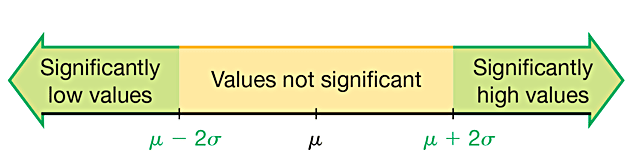
\includegraphics{pic9.png}
\item
  Using the 40 chocolate chip counts for the Chips Ahoy cookies, the mean is 24.0 chips and the standard deviation is 2.6 chips.

  \begin{itemize}
  \tightlist
  \item
    Use the range rule of thumb to find the minimum and maximum ``usual'' numbers of chips.\textbackslash{}
  \item
    Would a cookie with 30 chocolate chips be ``unusual''?
  \end{itemize}
\end{itemize}

\hypertarget{range-rule-of-thumb-for-estimating-a-value-of-the-standard-deviation-s}{%
\section{Range Rule of Thumb for Estimating a Value of the Standard Deviation s}\label{range-rule-of-thumb-for-estimating-a-value-of-the-standard-deviation-s}}

\begin{itemize}
\tightlist
\item
  To roughly estimate the standard deviation from a collection of known sample data use
  \[s\approx \frac{Range}{4}\]
  where range = (maximum value) - (minimum value)
\end{itemize}

\hypertarget{variance-of-a-sample-and-a-population}{%
\section{Variance of a Sample and a Population}\label{variance-of-a-sample-and-a-population}}

\begin{itemize}
\tightlist
\item
  The \textbf{variance} of a set of values is a measure of variation equal to the square of the standard deviation.

  \begin{itemize}
  \tightlist
  \item
    Sample variance: \(s^2\) - Square of the sample standard deviation \(s\)
  \item
    Population variance: \(\sigma^2\) - Square of the population standard deviation \(\sigma\)
  \item
    The units of the variance are the squares of the units of the original data values.
  \item
    The value of the variance can increase dramatically with the inclusion of outliers. (The variance is not resistant.)
  \item
    The value of the variance is never negative. It is zero only when all of the data values are the same number.
  \item
    The sample variance \(s^2\) is an unbiased estimator of the population variance \(\sigma^2\).
  \end{itemize}
\end{itemize}

\hypertarget{notations-1}{%
\section{Notations}\label{notations-1}}

\begin{itemize}
\tightlist
\item
  \(s\): samle standard deviation
\item
  \(n\): sample size
\item
  \(s^2\): sample variance
\item
  \(\sigma\): population standard deviation
\item
  \(N\): population size
\item
  \(\sigma^2\): population variance
\end{itemize}

\hypertarget{the-empirical-rule}{%
\section{The Empirical Rule}\label{the-empirical-rule}}

\begin{itemize}
\tightlist
\item
  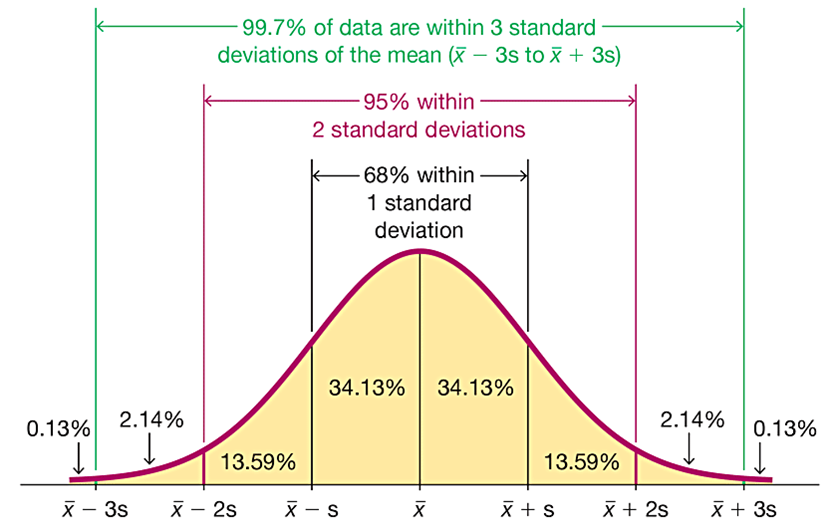
\includegraphics{pic10.png}
\item
  IQ scores have a bell-shaped distribution with a mean of 100 and a standard deviation of 15. What percentage of IQ scores are between 70 and 130?
\end{itemize}

\hypertarget{chebyshevs-theorem}{%
\section{Chebyshev's Theorem}\label{chebyshevs-theorem}}

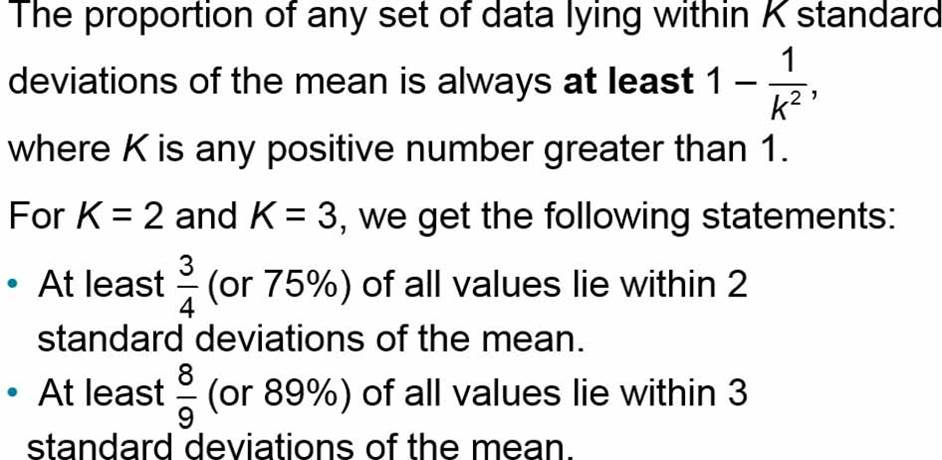
\includegraphics{pic11.jpg}

\hypertarget{extra-example}{%
\section{Extra Example}\label{extra-example}}

\begin{itemize}
\tightlist
\item
  A list has 10 numbers. Each number is a 1, 2, or 3. The average is 2 and the SD is 0. What is the list?
\end{itemize}

\hypertarget{measures-of-relative-standing-and-boxplots}{%
\section{Measures of Relative Standing and Boxplots}\label{measures-of-relative-standing-and-boxplots}}

\begin{itemize}
\tightlist
\item
  This section introduces measures of relative standing, which are numbers showing the location of data values relative to the other values within a data set.
\item
  They can be used to compare values from different data sets, or to compare values within the same data set.\\
\item
  The most important concept is the z score.
\item
  We will also discuss percentiles and quartiles, as well as a new statistical graph called the boxplot.
\end{itemize}

\hypertarget{z-scores}{%
\section{z Scores}\label{z-scores}}

\begin{itemize}
\tightlist
\item
  z-score (or standardized value) is the number of standard deviations that a given value x is above or below the mean.
\item
  z-score of a sample data value: \(z=\frac{x-\bar{x}}{s}\)
\item
  z-score of a population data value: \(z=\frac{x-\mu}{\sigma}\)
\item
  Round z scores to two decimal places
\end{itemize}

\hypertarget{important-properties-of-z-scores}{%
\section{Important Properties of z Scores}\label{important-properties-of-z-scores}}

\begin{itemize}
\tightlist
\item
  A z-score is the number of standard deviations that a given value x is above or below the mean.
\item
  z-scores are expressed as numbers with no units of measurement.
\item
  A data value is significantly low if its z-score is less than or equal to -2 or the value is significantly high if its z-score is greater than or equal to +2.
\item
  If an individual data value is less than the mean, its corresponding z score is a negative number.
\item
  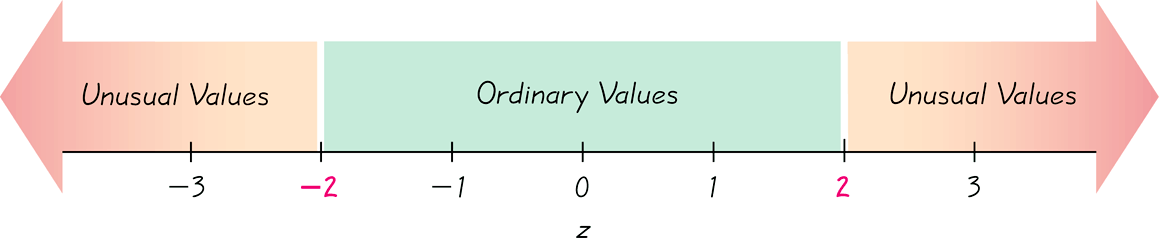
\includegraphics{pic12.png}
\end{itemize}

\hypertarget{examples}{%
\section{Examples}\label{examples}}

\begin{itemize}
\tightlist
\item
  Suppose the mean and standard deviation of a distribution are \(\mu=50\) and \(s = 5\)

  \begin{itemize}
  \tightlist
  \item
    If the x-value is 55, what is the z-score?
  \item
    If the x-value is 45, what is the z-score?
  \item
    If the x-value is 60, what is the z-score?
  \item
    So what does the z-score tell you?
  \item
    The author of the text measured his pulse rate to be 48 beats per minute. Is that pulse rate unusual if the mean adult male pulse rate is 67.3 beats per minute with a standard deviation of 10.3?
  \item
    Sally is taking two different math achievement tests with different means and standard deviations. The mean score on test A was 56 with a standard deviation of 3.5, while the mean score on test B was 65 with a standard deviation of 2.8. Sally scored a 62 on test A and a 69 on test B. On which test did Sally score the best? Why?
  \end{itemize}
\end{itemize}

\hypertarget{percentiles}{%
\section{Percentiles}\label{percentiles}}

\begin{itemize}
\tightlist
\item
  \textbf{Percentiles} are measures of location, denoted \(P_1\), \(P_2\), . . . , \(P_99\), which divide a set of data into 100 groups with about 1\% of the values in each group.
\item
  The process of finding the percentile that corresponds to a particular data value x is given by the following (round the result to the nearest whole number)
  \[\textrm{Percentile of a data value x}=\frac{\textrm{number of values less than x}}{\textrm{total number of values}}\times 100\]
\item
  The airport Verizon cell phone data speeds listed below are arranged in increasing order. Find the percentile for the data speed of 11.8 Mbps.
  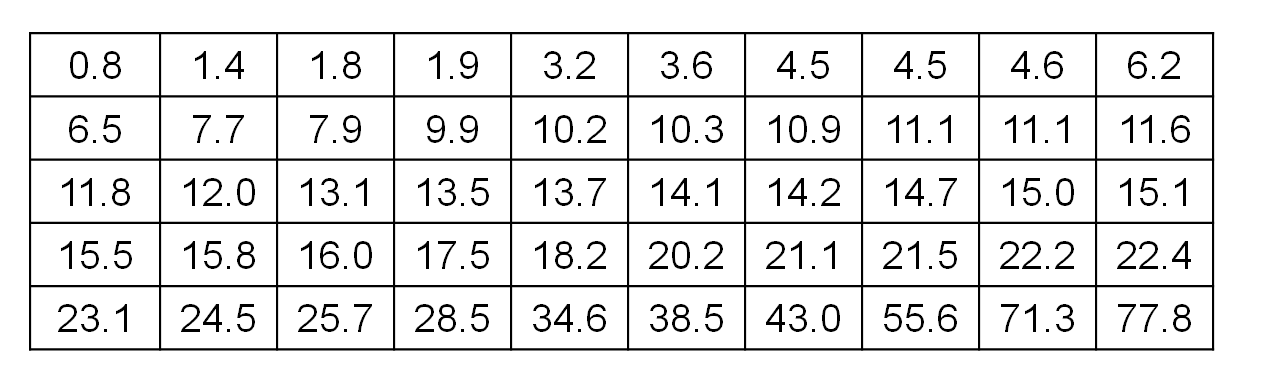
\includegraphics{pic13.png}
\end{itemize}

\hypertarget{interpretation-of-percentiles}{%
\section{Interpretation of Percentiles}\label{interpretation-of-percentiles}}

\begin{itemize}
\tightlist
\item
  From the previous example: A data speed of 11.8 Mbps is in the 40th percentile. This can be interpreted loosely as this:
  A data speed of 11.8 Mbps separates the lowest 40\% of values from the highest 60\% of values. We have \(P_{40} = 11.8\) Mbps.
\item
  Better interpretation: 40\% of the data values are less than 11.8 Mbps or 60\% of the data values are greater than 11.8 Mbps
\item
  What is the percentile for the median? How would you interpret the median better?
\end{itemize}

\hypertarget{example-from-a-dataset}{%
\section{Example from a dataset}\label{example-from-a-dataset}}

\begin{verbatim}
##   height ideal_ht sleep fastest
## 1     76       78   9.5     119
## 2     74       76   7.0     110
## 3     64       NA   9.0      85
## 4     62       65   7.0     100
## 5     72       72   8.0      95
\end{verbatim}

\begin{verbatim}
## 20% 50% 80% 90% 
##  90 102 120 130
\end{verbatim}

\begin{itemize}
\tightlist
\item
  Interpet the meanings of the above perentiles

  \begin{itemize}
  \tightlist
  \item
    About 20\% of the students drove slower than 90 mph
  \item
    About 50\% of the students drove slower than 102 mph (median!)
  \item
    About 80\% of the students drove slower than 120 mph
  \item
    About 90\% of the students drove slower than 130 mph
  \end{itemize}
\end{itemize}

\hypertarget{notations-2}{%
\section{Notations}\label{notations-2}}

\begin{itemize}
\tightlist
\item
  n total number of values in the data set
\item
  k percentile being used (Example: For the 25th percentile, k = 25.)
\item
  L locator that gives the position of a value (Example: For the 12th value in the sorted list, L = 12.)
\item
  \(P_k\) kth percentile (Example: \(P_{25}\) is the 25th percentile.)
\end{itemize}

\hypertarget{converting-a-percentile-to-a-data-value}{%
\section{Converting a Percentile to a Data Value}\label{converting-a-percentile-to-a-data-value}}

\begin{enumerate}
\def\labelenumi{\arabic{enumi}.}
\tightlist
\item
  Find L, where \(L=\frac{k}{100}\times n\)
\item
  If L is not a whole number, round up to the next whole number and find the data value in that position. If L is a whole number, average the data values in position L and L+1. (Notes: You need to put the numbers in order from small to large first.)
\end{enumerate}

\hypertarget{example-5}{%
\section{Example}\label{example-5}}

Refer to the sorted data speeds below. Find the 40th and 60th percentile, denoted by \(P_{40}\) and \(P_{60}\), respectively.

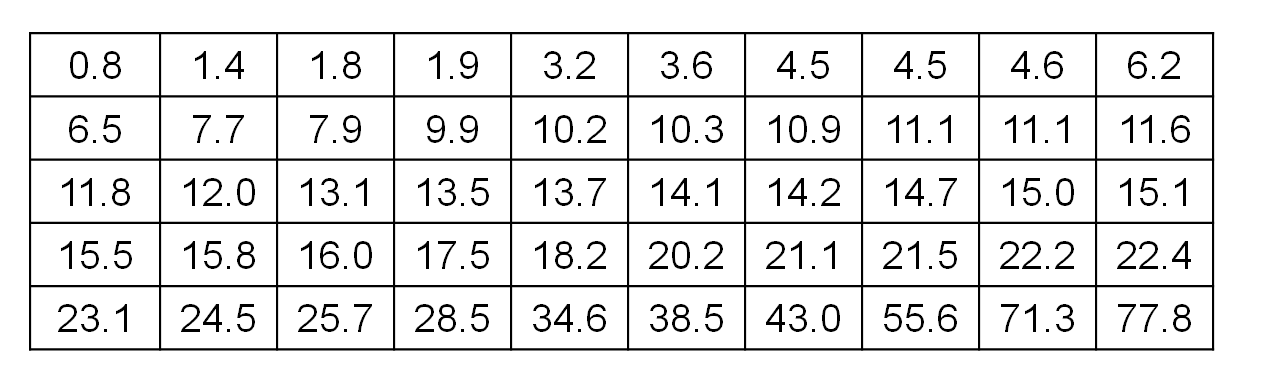
\includegraphics{pic13.png}

\hypertarget{quartiles}{%
\section{Quartiles}\label{quartiles}}

\begin{itemize}
\tightlist
\item
  Quartiles are measures of location, denoted \(Q_1\), \(Q_2\), and \(Q_3\), which divide a set of data into four groups with about 25\% of the values in each group
\item
  \(Q_1\) (First quartile): Same value as \(P_{25}\). It separates the bottom 25\% of the sorted values from the top 75\%.
\item
  \(Q_2\) (Second quartile): Same as \(P_{50}\) and same as the \textbf{median}. It separates the bottom 50\% of the sorted values from the top 50\%.
\item
  \(Q_3\) (Third quartile): Same as \(P_{75}\). It separates the bottom 75\% of the sorted values from the top 25\%.
\item
  Different technologies often yield different results.
\item
  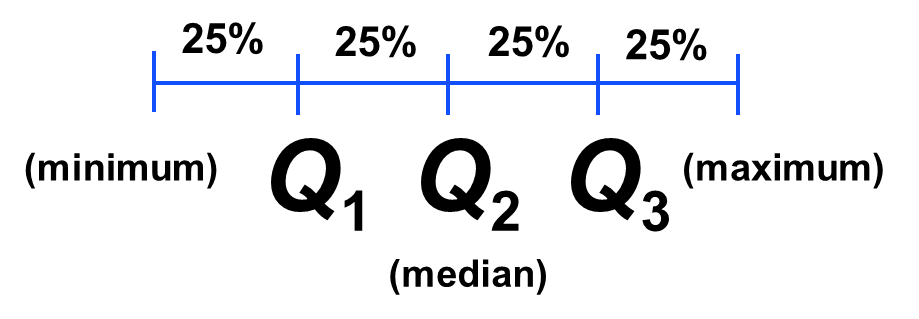
\includegraphics{pic14.png}
\end{itemize}

\hypertarget{statistics-defined-using-quartiles-and-percentiles}{%
\section{Statistics defined using quartiles and percentiles}\label{statistics-defined-using-quartiles-and-percentiles}}

Just focus on the Interquartile Range (IQR)
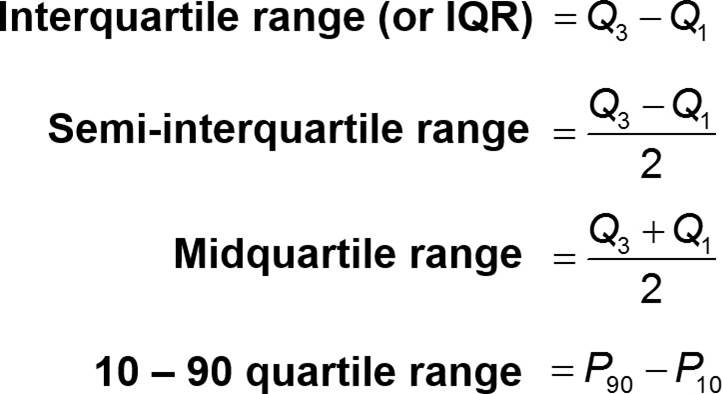
\includegraphics{pic15.jpg}

\hypertarget{number-summary}{%
\section{5-Number Summary}\label{number-summary}}

\begin{itemize}
\tightlist
\item
  For a set of data, the 5-number summary consists of these five values:

  \begin{itemize}
  \tightlist
  \item
    Minimum
  \item
    \(Q_1\)
  \item
    \(Q_2\) or median
  \item
    \(Q_3\)
  \item
    Maximum
  \end{itemize}
\end{itemize}

\hypertarget{example-finding-a-5-number-summary}{%
\section{Example: Finding a 5-Number Summary}\label{example-finding-a-5-number-summary}}

Use the Verizon airport data speeds to find the 5-number summary.

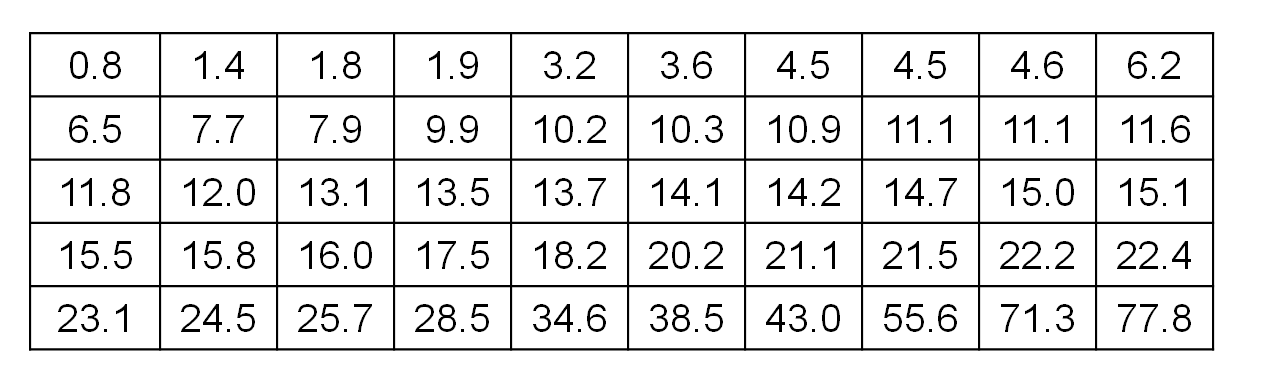
\includegraphics{pic13.png}

\hypertarget{boxplot-or-box-and-whisker-diagram}{%
\section{Boxplot (or Box-and-Whisker Diagram)}\label{boxplot-or-box-and-whisker-diagram}}

\begin{itemize}
\tightlist
\item
  A boxplot (or box-and-whisker diagram) is a graph of a data set that consists of a line extending from the minimum value to the maximum value, and a box with lines drawn at the first quartile \(Q_1\), the median, and the third quartile \(Q_3\).
\end{itemize}

\hypertarget{procedure-for-constructing-a-boxplot}{%
\section{Procedure for Constructing a Boxplot}\label{procedure-for-constructing-a-boxplot}}

\begin{enumerate}
\def\labelenumi{\arabic{enumi}.}
\tightlist
\item
  Find the 5-number summary (minimum value, \(Q_1\), \(Q_2\), \(Q_3\), maximum value).
\item
  Construct a line segment extending from the minimum data value to the maximum data value.
\item
  Construct a box (rectangle) extending from Q1 to Q3, and draw a line in the box at the value of Q2 (median).
\end{enumerate}

\begin{itemize}
\tightlist
\item
  Use the Verizon airport data speeds to construct a boxplot.
\item
  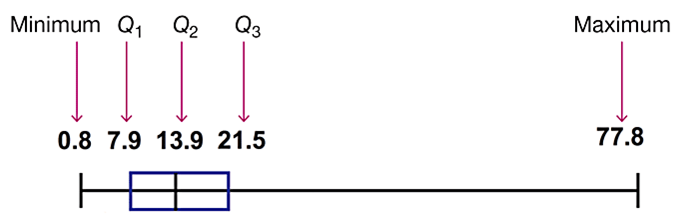
\includegraphics{pic15.png}
\end{itemize}

\hypertarget{skewness}{%
\section{Skewness}\label{skewness}}

\begin{itemize}
\tightlist
\item
  A boxplot can often be used to identify skewness. A distribution of data is skewed if it is not symmetric and extends more to one side than to the other.
\item
  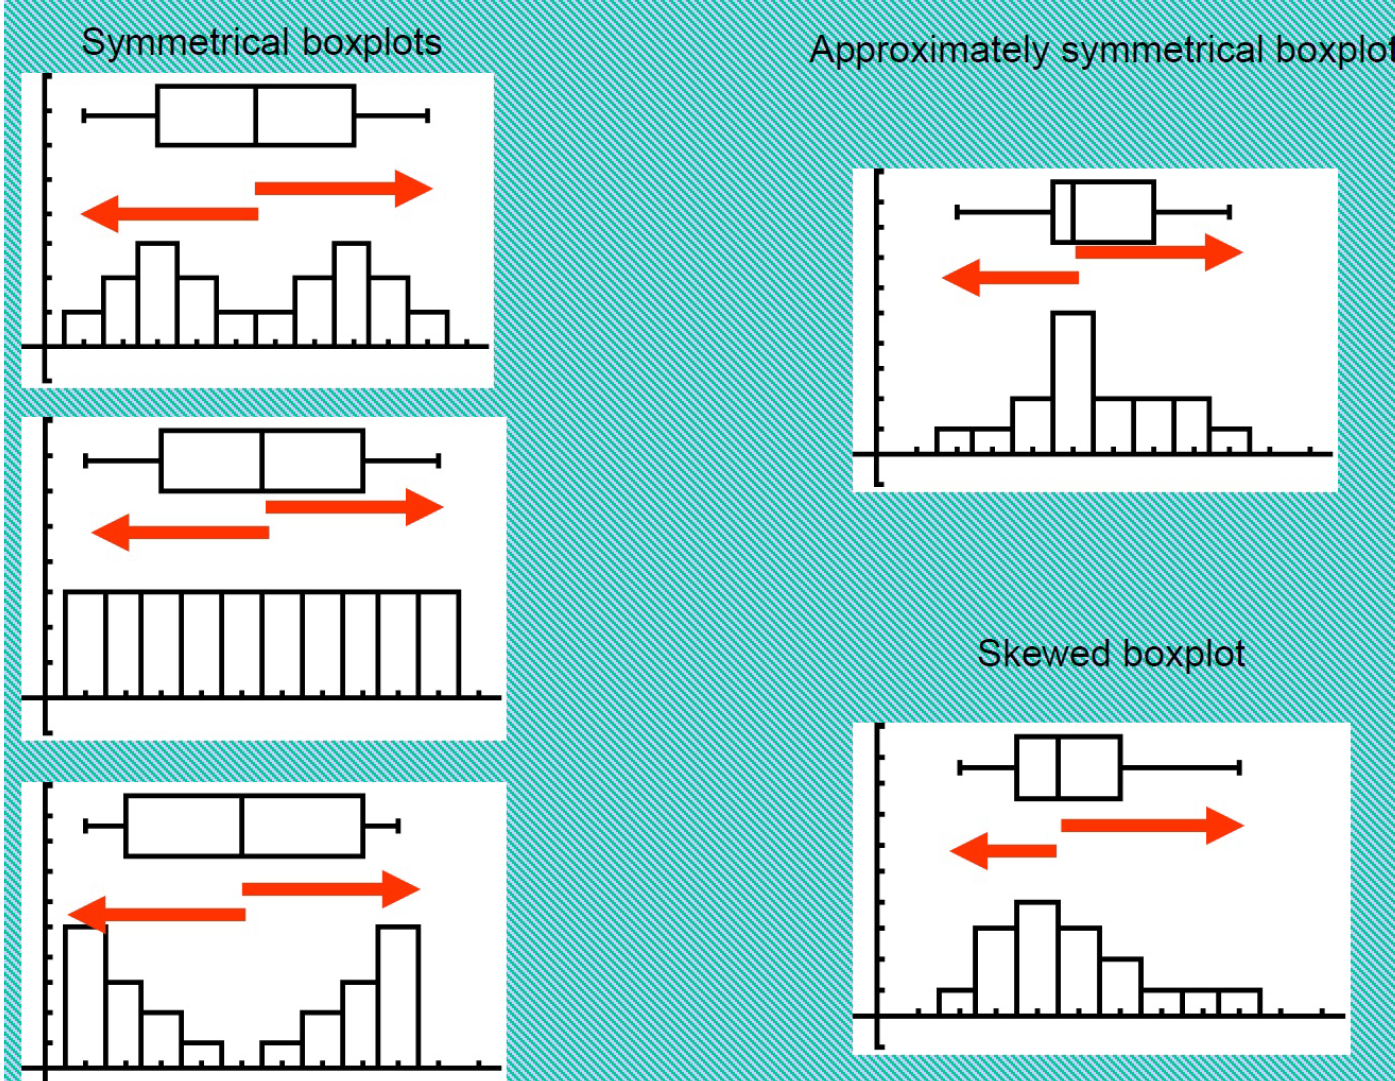
\includegraphics{pic16.png}
\end{itemize}

\hypertarget{identifying-outliers-for-modified-boxplots}{%
\section{Identifying Outliers for Modified Boxplots}\label{identifying-outliers-for-modified-boxplots}}

\begin{enumerate}
\def\labelenumi{\arabic{enumi}.}
\tightlist
\item
  Find the quartiles \(Q_1\), \(Q_2\), and \(Q_3\).
\item
  Find the interquartile range (IQR), where \(\textrm{IQR} = Q_3- Q_1\).
\item
  Evaluate \(1.5\times \textrm{IQR}\).
\item
  In a modified boxplot, a data value is an outlier if it is above \(Q_3\), by an amount greater than \(1.5\times \textrm{IQR}\) or below \(Q_1\), by an amount greater than \(1.5\times \textrm{IQR}\).
\end{enumerate}

\hypertarget{modified-boxplot}{%
\section{Modified Boxplot}\label{modified-boxplot}}

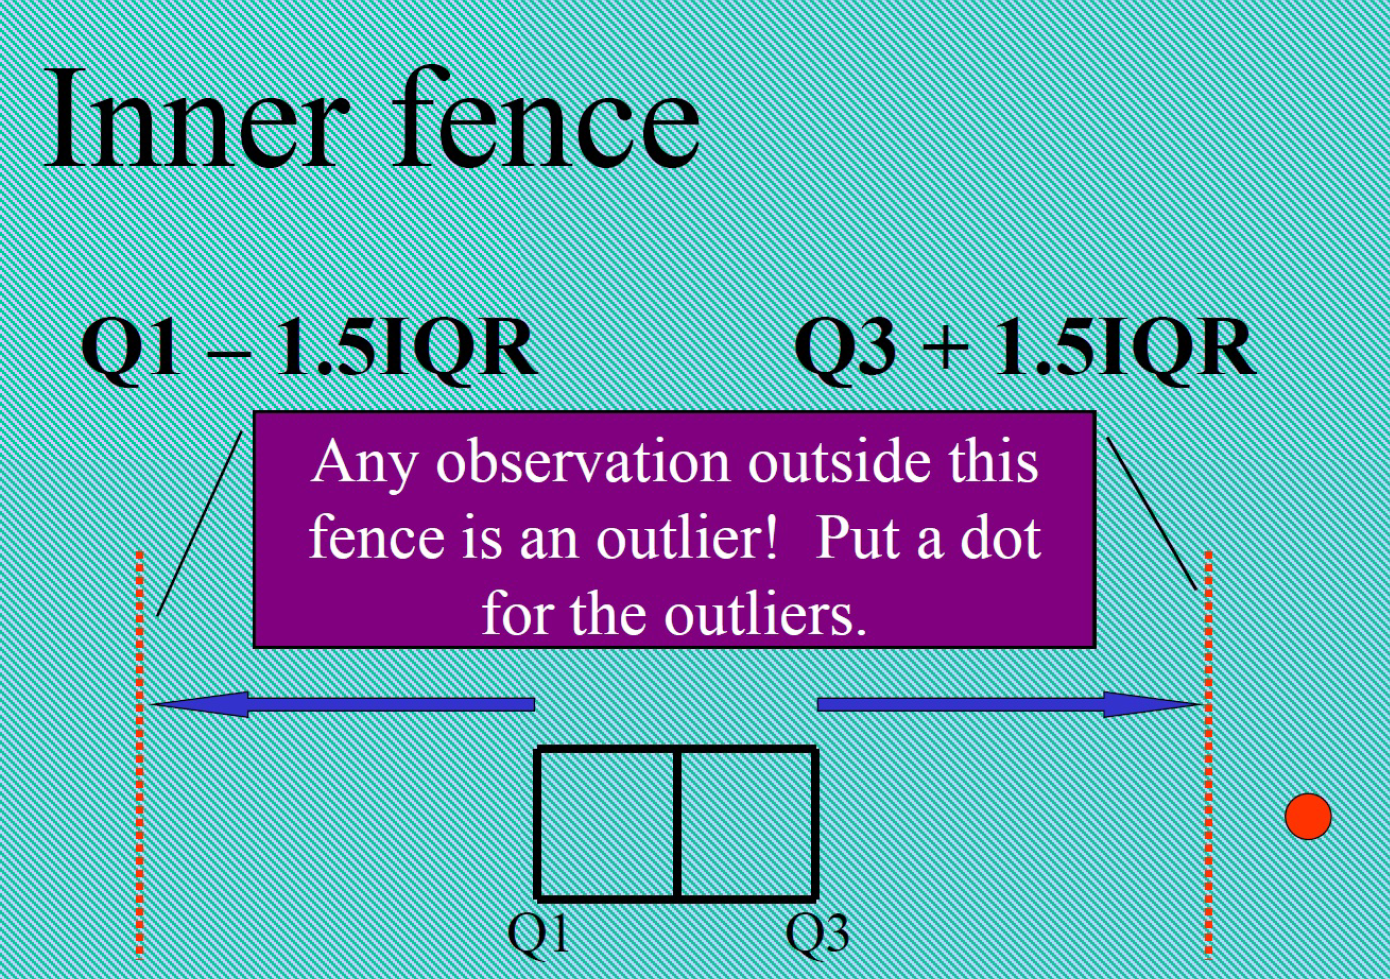
\includegraphics{pic17.png}

\hypertarget{example-6}{%
\section{Example}\label{example-6}}

\begin{verbatim}
##  min  Q1 median Q3 max mean sd  n missing
##  0.8 8.4     14 21  78   18 16 50       0
\end{verbatim}

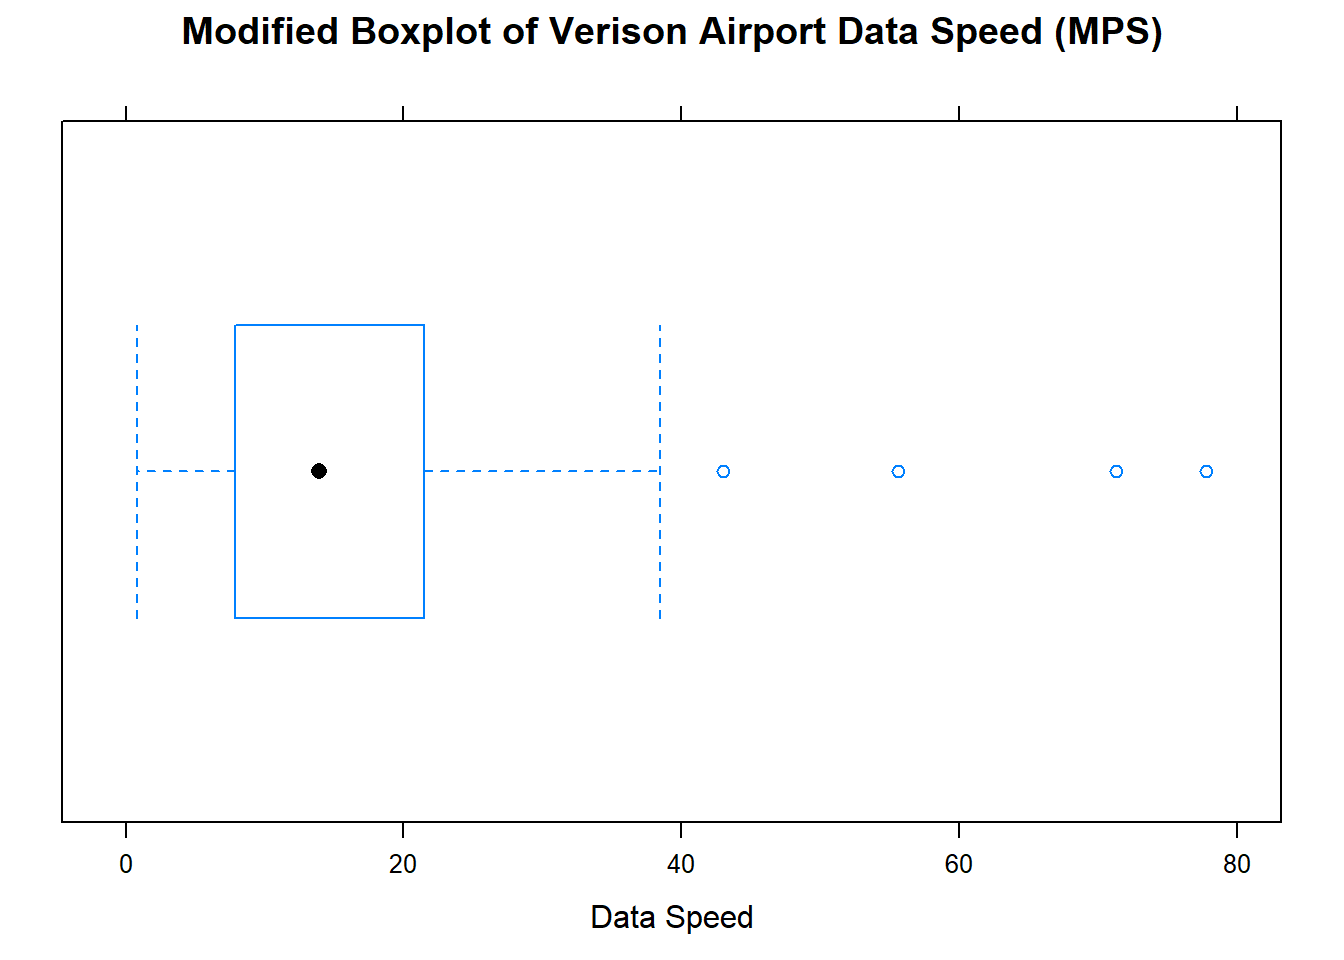
\includegraphics{Book_files/figure-latex/unnamed-chunk-9-1.pdf}

\begin{verbatim}
## $stats
## [1]  0.8  7.9 13.9 21.5 38.5
## 
## $n
## [1] 50
## 
## $conf
## [1] 11 17
## 
## $out
## [1] 43 56 71 78
\end{verbatim}

\hypertarget{comparative-boxplots}{%
\section{Comparative Boxplots}\label{comparative-boxplots}}

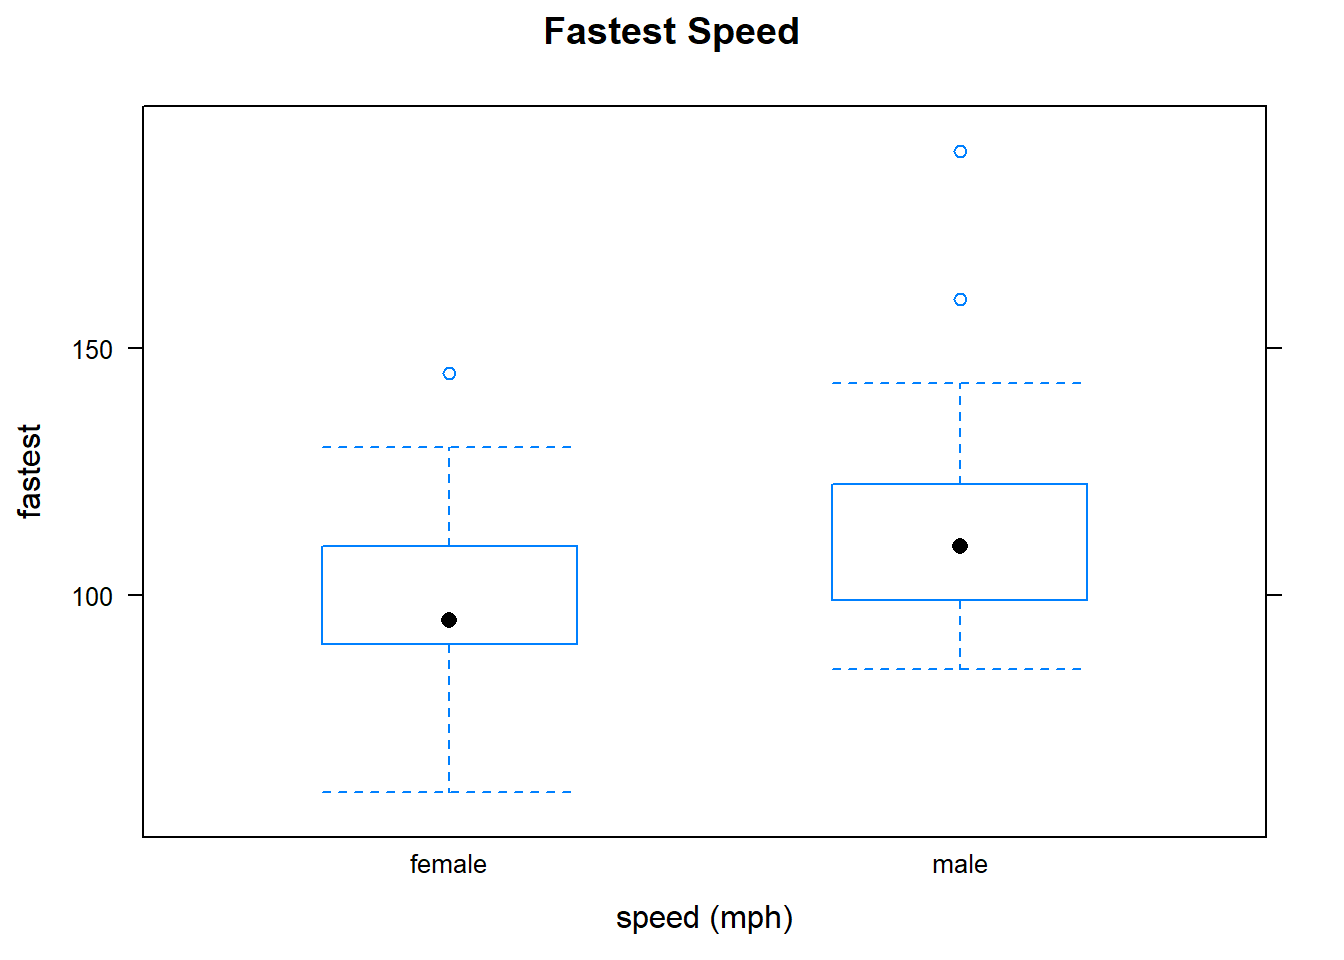
\includegraphics{Book_files/figure-latex/unnamed-chunk-10-1.pdf}

\hypertarget{methods}{%
\chapter{Methods}\label{methods}}

We describe our methods in this chapter.

\hypertarget{applications}{%
\chapter{Applications}\label{applications}}

Some \emph{significant} applications are demonstrated in this chapter.

\hypertarget{example-one}{%
\section{Example one}\label{example-one}}

\hypertarget{example-two}{%
\section{Example two}\label{example-two}}

\hypertarget{final-words}{%
\chapter{Final Words}\label{final-words}}

We have finished a nice book.

\bibliography{book.bib,packages.bib}


\end{document}
